% !TEX program = xelatex
\documentclass[UTF8,fontset=fandol,a4paper,11pt]{ctexart}
\usepackage[margin=21mm,top=23mm,bottom=22mm,headheight=16pt]{geometry}
\usepackage{amsmath,amssymb,mathtools,bm}
\usepackage{tikz}
\usetikzlibrary{arrows.meta,calc,angles,quotes,patterns}
\usepackage{xcolor,booktabs,array,longtable,enumitem,fancyhdr,needspace}
\usepackage[unicode,hidelinks]{hyperref}
\definecolor{ink}{HTML}{24343C}
\definecolor{accent}{HTML}{166A70}
\definecolor{muted}{HTML}{65747A}
\definecolor{rulegray}{HTML}{D4DDE0}
\definecolor{warm}{HTML}{966037}
\color{ink}
\setlength{\parindent}{2em}
\setlength{\parskip}{4pt}
\linespread{1.12}
\AtBeginDocument{\setlength{\abovedisplayskip}{6pt plus 2pt minus 1pt}
\setlength{\belowdisplayskip}{6pt plus 2pt minus 1pt}
\setlength{\abovedisplayshortskip}{0pt plus 1pt}
\setlength{\belowdisplayshortskip}{4pt plus 1pt}}
\setlist[enumerate]{label=(\arabic*),leftmargin=2.3em,itemsep=3pt,topsep=4pt}
\setlist[itemize]{leftmargin=2em,itemsep=2pt,topsep=4pt}
\allowdisplaybreaks[1]
\setlength{\emergencystretch}{2em}
\setcounter{secnumdepth}{0}
\providecommand{\tightlist}{\setlength{\itemsep}{0pt}\setlength{\parskip}{0pt}}
\ctexset{section={format=\Large\bfseries\color{accent},beforeskip=10pt,afterskip=9pt},
subsection={format=\normalsize\bfseries\color{accent},beforeskip=10pt,afterskip=4pt},
subsubsection={format=\normalsize\bfseries,beforeskip=8pt,afterskip=3pt}}
\pagestyle{fancy}
\fancyhf{}
\fancyhead[L]{\small\color{muted}物理学难题集萃}
% 页眉仅保留书名；版本名称只在封面显示。
\fancyfoot[L]{\small\color{muted}\chapterlabel}
\fancyfoot[R]{\small\thepage}
\renewcommand{\headrulewidth}{0.4pt}
\renewcommand{\footrulewidth}{0pt}
\newcommand{\dd}{\mathop{}\!\mathrm{d}}
\newcommand{\vect}[1]{\bm{#1}}
\newcommand{\tagline}[1]{\noindent{\small\color{muted}#1}\par}
\newcommand{\result}[1]{\begin{equation*}\boxed{#1}\end{equation*}}
\newcommand{\figcaption}[1]{\par\vspace{2pt}{\small\color{muted}#1}\par}
\newcommand{\teach}[2]{\Needspace{4\baselineskip}\subsection*{讲解要点与追问}#1\par\smallskip\noindent\textbf{追问：}#2\par}
\newcommand{\workarea}{\par\vspace{7mm}\noindent{\small\color{muted}作答区}\par\vspace{4mm}
\noindent\textcolor{rulegray}{\rule{\linewidth}{0.3pt}}\par\vspace{16mm}
\noindent\textcolor{rulegray}{\rule{\linewidth}{0.3pt}}\par\vspace{16mm}
\noindent\textcolor{rulegray}{\rule{\linewidth}{0.3pt}}\par\vspace{16mm}
\noindent\textcolor{rulegray}{\rule{\linewidth}{0.3pt}}}
\tikzset{axis/.style={-{Stealth[length=2mm]},thin,color=muted},
motion/.style={-{Stealth[length=2.3mm]},thick,color=accent},
force/.style={-{Stealth[length=2.3mm]},thick,color=warm},
traj/.style={thick,color=accent},guide/.style={dashed,thin,color=muted},
object/.style={thick,color=ink},every node/.style={font=\small}}\widowpenalty=10000\clubpenalty=10000\displaywidowpenalty=10000\newcommand{\chapterlabel}{热学试题（二）}







\hypersetup{pdftitle={热学试题（二）·学生解答版},pdfauthor={}}

\begin{document}\pdfbookmark[0]{热学试题（二）}{cover}

\thispagestyle{empty}\vspace*{22mm}

\noindent{\Huge\bfseries 物理学难题集萃}\par\vspace{12mm}

\noindent{\LARGE 热学试题（二）}\par\vspace{12mm}

\noindent{\Large\color{accent}学生解答版}\par\vspace{9mm}

\noindent\textcolor{accent}{\rule{\linewidth}{1pt}}\par\vspace{9mm}

\noindent 第1--5题\par\vfill\clearpage

\pdfbookmark[1]{题目目录}{contents}\section*{题目目录}

\begin{longtable}{@{}r p{113mm} r@{}}\toprule 题号 & 题目 & 页码\\\midrule

\hyperref[q:1]{1} & \hyperref[q:1]{热容量阶跃下的矩形循环} & \pageref{q:1} \\

\hyperref[q:2]{2} & \hyperref[q:2]{有限热源的最大作功与相变卡诺循环} & \pageref{q:2} \\

\hyperref[q:3]{3} & \hyperref[q:3]{从活塞与分子碰撞导出绝热方程} & \pageref{q:3} \\

\hyperref[q:4]{4} & \hyperref[q:4]{导热稳态、分子扩散与撤热源后的平衡} & \pageref{q:4} \\

\hyperref[q:5]{5} & \hyperref[q:5]{光子气体的压强、绝热关系与辐射能流} & \pageref{q:5} \\

\bottomrule\end{longtable}

\clearpage

\pdfbookmark[2]{第 1 题 热容量阶跃下的矩形循环}{q1}

\section*{第 1 题\quad 热容量阶跃下的矩形循环}\label{q:1}


$\nu$ mol理想气体的定体摩尔热容量为
\[
C_V(T)=
\begin{cases}
\alpha R,&T<2T_0,\\
\alpha\beta R,&T>2T_0,
\end{cases}
\qquad \alpha>1,\quad\beta>1.
\]
气体内能由给定热容量连续积分确定，取$U(0)=0$。气体经历图热试2.1所示的顺时针矩形循环$A\to B\to C\to D\to A$，其中$AB,CD$等体，$BC,DA$等压，已知$T_A=T_0,T_B=2T_0,T_C=3T_0$。
\begin{enumerate}
\item 求$T_D$，画$U$--$T$关系，并在图中标出四态及$CD$上$T=2T_0$的状态$E$。
\item 求循环效率；说明热容量的阶跃是否足以引入定温吸放热。
\end{enumerate}


\begin{center}\begin{minipage}{.98\linewidth}\centering
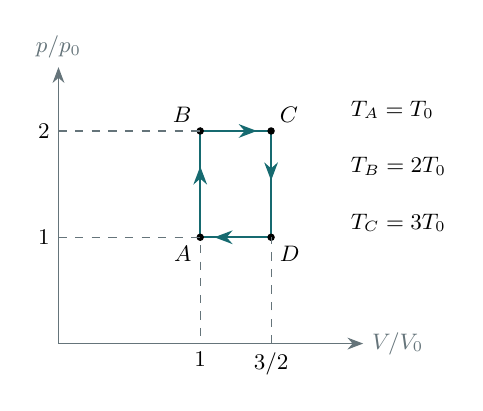
\begin{tikzpicture}[scale=.9,transform shape]

\draw[axis] (0,0)--(4.3,0) node[right] {$V/V_0$};
\draw[axis] (0,0)--(0,3.9) node[above] {$p/p_0$};
\draw[traj] (2,1.5)--(2,3)--(3,3)--(3,1.5)--cycle;
\draw[motion] (2,1.9)--(2,2.5);
\draw[motion] (2.2,3)--(2.8,3);
\draw[motion] (3,2.7)--(3,2.3);
\draw[motion] (2.8,1.5)--(2.2,1.5);
\foreach \x/\y/\lab/\pos in {2/1.5/A/below left,2/3/B/above left,3/3/C/above right,3/1.5/D/below right}{
\fill (\x,\y) circle (1.5pt) node[\pos] {$\lab$};}
\node[below] at (2,0) {$1$};\node[below] at (3,0) {$3/2$};
\node[left] at (0,1.5) {$1$};\node[left] at (0,3) {$2$};
\draw[guide] (0,1.5)--(2,1.5)--(2,0);
\draw[guide] (0,3)--(2,3);\draw[guide] (3,0)--(3,1.5);

\node[right] at (4,3.3) {$T_A=T_0$};
\node[right] at (4,2.5) {$T_B=2T_0$};
\node[right] at (4,1.7) {$T_C=3T_0$};

\end{tikzpicture}
\figcaption{图热试2.1\quad 顺时针矩形循环；体积与压强坐标按初态归一化。}
\end{minipage}\end{center}

\Needspace{6\baselineskip}\subsection*{解答}


图热试2.1中取$A$态压强、体积为$p_0,V_0$，满足$p_0V_0=\nu RT_0$。由$AB$等体且$T_B=2T_0$，得$p_B=2p_0$；$BC$等压且$T_C=3T_0$，得$V_C=3V_0/2$。于是
\[
D:\quad p_D=p_0,\quad V_D=\frac32V_0,
\qquad
\boxed{T_D=\frac32T_0}.
\]
在$CD$上$V=3V_0/2$不变，因此$T_E=2T_0$处$p_E=4p_0/3$。

$E$与$B$有同一温度，但等体线不同：$E$在右侧的$V=3V_0/2$上，$B$在左侧的$V=V_0$上。矩形路径的各态依次为$(p/p_0,V/V_0)=(1,1),(2,1),(2,3/2),(1,3/2)$，对应温度依次为$1,2,3,3/2$倍$T_0$。由热容量定义$\mathrm dU=\nu C_V(T)\,\mathrm dT$，应从零温基准分段积分：
\[
U(T)=
\begin{cases}
\alpha\nu RT,&0\le T\le2T_0,\\[2pt]
2\alpha\nu RT_0+\alpha\beta\nu R(T-2T_0),&T\ge2T_0.
\end{cases}
\]
具体地，低温段从$U(0)=0$积到$U(2T_0)=\nu\int_0^{2T_0}\alpha R\mathrm dT$。高温段再从这个值继续累积$\nu\int_{2T_0}^T\alpha\beta R\mathrm dT$，于是斜率变为$\alpha\beta\nu R$，连接温度的内能值仍由前段确定。两段在$2T_0$处都等于$2\alpha\nu RT_0$，所以内能连续，只有斜率发生改变。高温段保留低温积分累积的$2\alpha\nu RT_0$，并从$2T_0$开始按新热容量继续积分，所以两段的积分常数彼此匹配。
\begin{center}\begin{minipage}{.98\linewidth}\centering
\begin{tikzpicture}[scale=.8,transform shape]
\draw[axis] (0,0)--(10.7,0) node[right] {$T/T_0$};
\draw[axis] (0,0)--(0,3.2) node[above] {$U/(\alpha\nu RT_0)$};
\node[above] at (5,3.5) {$\beta=2$示例：内能在温度2处连续};
\draw[traj] plot coordinates {(0.000000000,0.000000000) (0.064000000,0.014000000) (0.128000000,0.028000000) (0.192000000,0.042000000) (0.256000000,0.056000000) (0.320000000,0.070000000) (0.384000000,0.084000000) (0.448000000,0.098000000) (0.512000000,0.112000000) (0.576000000,0.126000000) (0.640000000,0.140000000) (0.704000000,0.154000000) (0.768000000,0.168000000) (0.832000000,0.182000000) (0.896000000,0.196000000) (0.960000000,0.210000000) (1.024000000,0.224000000) (1.088000000,0.238000000) (1.152000000,0.252000000) (1.216000000,0.266000000) (1.280000000,0.280000000) (1.344000000,0.294000000) (1.408000000,0.308000000) (1.472000000,0.322000000) (1.536000000,0.336000000) (1.600000000,0.350000000) (1.664000000,0.364000000) (1.728000000,0.378000000) (1.792000000,0.392000000) (1.856000000,0.406000000) (1.920000000,0.420000000) (1.984000000,0.434000000) (2.048000000,0.448000000) (2.112000000,0.462000000) (2.176000000,0.476000000) (2.240000000,0.490000000) (2.304000000,0.504000000) (2.368000000,0.518000000) (2.432000000,0.532000000) (2.496000000,0.546000000) (2.560000000,0.560000000) (2.624000000,0.574000000) (2.688000000,0.588000000) (2.752000000,0.602000000) (2.816000000,0.616000000) (2.880000000,0.630000000) (2.944000000,0.644000000) (3.008000000,0.658000000) (3.072000000,0.672000000) (3.136000000,0.686000000) (3.200000000,0.700000000) (3.264000000,0.714000000) (3.328000000,0.728000000) (3.392000000,0.742000000) (3.456000000,0.756000000) (3.520000000,0.770000000) (3.584000000,0.784000000) (3.648000000,0.798000000) (3.712000000,0.812000000) (3.776000000,0.826000000) (3.840000000,0.840000000) (3.904000000,0.854000000) (3.968000000,0.868000000) (4.032000000,0.882000000) (4.096000000,0.896000000) (4.160000000,0.910000000) (4.224000000,0.924000000) (4.288000000,0.938000000) (4.352000000,0.952000000) (4.416000000,0.966000000) (4.480000000,0.980000000) (4.544000000,0.994000000) (4.608000000,1.008000000) (4.672000000,1.022000000) (4.736000000,1.036000000) (4.800000000,1.050000000) (4.864000000,1.064000000) (4.928000000,1.078000000) (4.992000000,1.092000000) (5.056000000,1.106000000) (5.120000000,1.120000000) (5.184000000,1.134000000) (5.248000000,1.148000000) (5.312000000,1.162000000) (5.376000000,1.176000000) (5.440000000,1.190000000) (5.504000000,1.204000000) (5.568000000,1.218000000) (5.632000000,1.232000000) (5.696000000,1.246000000) (5.760000000,1.260000000) (5.824000000,1.274000000) (5.888000000,1.288000000) (5.952000000,1.302000000) (6.016000000,1.316000000) (6.080000000,1.330000000) (6.144000000,1.344000000) (6.208000000,1.358000000) (6.272000000,1.372000000) (6.336000000,1.386000000) (6.400000000,1.400000000) (6.464000000,1.428000000) (6.528000000,1.456000000) (6.592000000,1.484000000) (6.656000000,1.512000000) (6.720000000,1.540000000) (6.784000000,1.568000000) (6.848000000,1.596000000) (6.912000000,1.624000000) (6.976000000,1.652000000) (7.040000000,1.680000000) (7.104000000,1.708000000) (7.168000000,1.736000000) (7.232000000,1.764000000) (7.296000000,1.792000000) (7.360000000,1.820000000) (7.424000000,1.848000000) (7.488000000,1.876000000) (7.552000000,1.904000000) (7.616000000,1.932000000) (7.680000000,1.960000000) (7.744000000,1.988000000) (7.808000000,2.016000000) (7.872000000,2.044000000) (7.936000000,2.072000000) (8.000000000,2.100000000) (8.064000000,2.128000000) (8.128000000,2.156000000) (8.192000000,2.184000000) (8.256000000,2.212000000) (8.320000000,2.240000000) (8.384000000,2.268000000) (8.448000000,2.296000000) (8.512000000,2.324000000) (8.576000000,2.352000000) (8.640000000,2.380000000) (8.704000000,2.408000000) (8.768000000,2.436000000) (8.832000000,2.464000000) (8.896000000,2.492000000) (8.960000000,2.520000000) (9.024000000,2.548000000) (9.088000000,2.576000000) (9.152000000,2.604000000) (9.216000000,2.632000000) (9.280000000,2.660000000) (9.344000000,2.688000000) (9.408000000,2.716000000) (9.472000000,2.744000000) (9.536000000,2.772000000) (9.600000000,2.800000000)};
\node[below] at (0,-.12) {$0$};
\node[below] at (3.2,-.12) {$1$};
\node[below] at (4.8,-.12) {$3/2$};
\node[below] at (6.4,-.12) {$2$};
\node[below] at (9.6,-.12) {$3$};
\fill (3.2,.7) circle(.04) node[above left] {$A$};\fill (4.8,1.05) circle(.04) node[below right] {$D$};\fill (6.4,1.4) circle(.04) node[above left] {$B,E$};\fill (9.6,2.8) circle(.04) node[above] {$C$};\end{tikzpicture}
\figcaption{解图热试2.1A\quad $\beta=2$示例：内能在温度2处连续}
\end{minipage}\end{center}
解图热试2.1A以$t=T/T_0$、$u=U/(\alpha\nu RT_0)$为坐标，折线为
\[
u=t\quad(t\le2),\qquad u=2+\beta(t-2)\quad(t\ge2).
\]
四态的内能分别为
\[
U_A=\alpha\nu RT_0,\quad U_B=2\alpha\nu RT_0,\quad
U_C=\alpha(\beta+2)\nu RT_0,\quad
U_D=\frac32\alpha\nu RT_0.
\]
$B,E$在$U$--$T$图上重合，但$V_B=V_0$、$V_E=3V_0/2$，在$p$--$V$图上是两个状态；理想气体的内能只由温度确定，体积与压强还由状态方程及所在过程分别确定。

\begin{center}\begin{minipage}{.98\linewidth}\centering
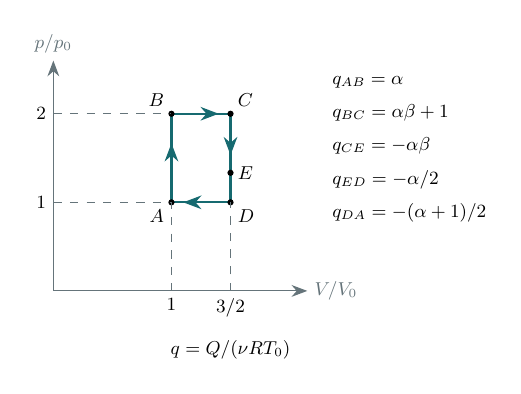
\begin{tikzpicture}[scale=.75,transform shape]

\draw[axis] (0,0)--(4.3,0) node[right] {$V/V_0$};
\draw[axis] (0,0)--(0,3.9) node[above] {$p/p_0$};
\draw[traj] (2,1.5)--(2,3)--(3,3)--(3,1.5)--cycle;
\draw[motion] (2,1.9)--(2,2.5);
\draw[motion] (2.2,3)--(2.8,3);
\draw[motion] (3,2.7)--(3,2.3);
\draw[motion] (2.8,1.5)--(2.2,1.5);
\foreach \x/\y/\lab/\pos in {2/1.5/A/below left,2/3/B/above left,3/3/C/above right,3/1.5/D/below right}{
\fill (\x,\y) circle (1.5pt) node[\pos] {$\lab$};}
\node[below] at (2,0) {$1$};\node[below] at (3,0) {$3/2$};
\node[left] at (0,1.5) {$1$};\node[left] at (0,3) {$2$};
\draw[guide] (0,1.5)--(2,1.5)--(2,0);
\draw[guide] (0,3)--(2,3);\draw[guide] (3,0)--(3,1.5);

\fill (3,2) circle (1.5pt) node[right] {$E$};
\node[align=left,right] at (4.6,2.4) {$q_{AB}=\alpha$\\[5pt]$q_{BC}=\alpha\beta+1$\\[5pt]$q_{CE}=-\alpha\beta$\\[5pt]$q_{ED}=-\alpha/2$\\[5pt]$q_{DA}=-(\alpha+1)/2$};
\node at (3,-1) {$q=Q/(\nu RT_0)$};

\end{tikzpicture}
\figcaption{解图热试2.1B\quad 冷却在E处分段，各段热量之和等于矩形面积功。}
\end{minipage}\end{center}
图A的两段直线以$\beta=2$示例，低温斜率为1，高温斜率为2；一般$\beta$只改变高温段斜率。沿$AB$逐渐升温时，内能图上的点从$A$走向$B$；沿$CD$逐渐降温时，从$C$经与$B$重合的$E$走向$D$。$D$也与$AB$上某状态投影重合，因为它们温度相同；各态在完整$p$—$V$空间中的位置由不同等体线区分。

解图热试2.1B将$CD$的冷却按$E$分开，用各段正确热容量计算。以下以$q=Q/(\nu RT_0)$表示代数热量，吸热为正：
\[
q_{AB}=\alpha,\qquad
q_{BC}=\alpha\beta+1.
\]
其中$BC$有$\Delta U=\alpha\beta\nu RT_0$，还做功$2p_0(V_0/2)=\nu RT_0$。在$CD$上先由$3T_0$降到$2T_0$，再由$2T_0$降到$3T_0/2$，故
\[
q_{CD}=-\alpha\beta-\frac12\alpha,
\qquad
q_{DA}=-\frac12(\alpha+1).
\]
$DA$的内能变化为$-\alpha\nu RT_0/2$，压缩功为$-p_0V_0/2$。冷却的两段分别有$q_{CE}=-\alpha\beta$与$q_{ED}=-\alpha/2$；它们温降分别为$T_0$与$T_0/2$，均为负热量。$AB$与$BC$的代数热量为正，$CD$与$DA$为负，因此正吸热量取前两项之和，正放热量取后两项相反数之和。合计正吸热量、正放热量与净功：
\[
Q_{\rm in}=[\alpha(1+\beta)+1]\nu RT_0,
\]
\[
Q_{\rm out}=\left[\alpha(1+\beta)+\frac12\right]\nu RT_0,
\qquad
W_{\rm cyc}=\frac12\nu RT_0.
\]
净功也等于$p$--$V$矩形面积
\[
(2p_0-p_0)\left(\frac32V_0-V_0\right)
=\frac12p_0V_0,
\]
因此
\[
\boxed{\eta=\frac1{2[\alpha(1+\beta)+1]}}.
\]
\begin{center}\begin{minipage}{.98\linewidth}\centering
\begin{tikzpicture}[scale=.8,transform shape]
\draw[axis] (0,0)--(10.7,0) node[right] {$\beta$};
\draw[axis] (0,0)--(0,3.2) node[above] {$\eta$};
\node[above] at (5,3.5) {$\alpha=2$：矩形功固定，吸热增大};
\draw[traj] plot coordinates {(0.000000000,2.800000000) (0.083333333,2.763157895) (0.166666667,2.727272727) (0.250000000,2.692307692) (0.333333333,2.658227848) (0.416666667,2.625000000) (0.500000000,2.592592593) (0.583333333,2.560975610) (0.666666667,2.530120482) (0.750000000,2.500000000) (0.833333333,2.470588235) (0.916666667,2.441860465) (1.000000000,2.413793103) (1.083333333,2.386363636) (1.166666667,2.359550562) (1.250000000,2.333333333) (1.333333333,2.307692308) (1.416666667,2.282608696) (1.500000000,2.258064516) (1.583333333,2.234042553) (1.666666667,2.210526316) (1.750000000,2.187500000) (1.833333333,2.164948454) (1.916666667,2.142857143) (2.000000000,2.121212121) (2.083333333,2.100000000) (2.166666667,2.079207921) (2.250000000,2.058823529) (2.333333333,2.038834951) (2.416666667,2.019230769) (2.500000000,2.000000000) (2.583333333,1.981132075) (2.666666667,1.962616822) (2.750000000,1.944444444) (2.833333333,1.926605505) (2.916666667,1.909090909) (3.000000000,1.891891892) (3.083333333,1.875000000) (3.166666667,1.858407080) (3.250000000,1.842105263) (3.333333333,1.826086957) (3.416666667,1.810344828) (3.500000000,1.794871795) (3.583333333,1.779661017) (3.666666667,1.764705882) (3.750000000,1.750000000) (3.833333333,1.735537190) (3.916666667,1.721311475) (4.000000000,1.707317073) (4.083333333,1.693548387) (4.166666667,1.680000000) (4.250000000,1.666666667) (4.333333333,1.653543307) (4.416666667,1.640625000) (4.500000000,1.627906977) (4.583333333,1.615384615) (4.666666667,1.603053435) (4.750000000,1.590909091) (4.833333333,1.578947368) (4.916666667,1.567164179) (5.000000000,1.555555556) (5.083333333,1.544117647) (5.166666667,1.532846715) (5.250000000,1.521739130) (5.333333333,1.510791367) (5.416666667,1.500000000) (5.500000000,1.489361702) (5.583333333,1.478873239) (5.666666667,1.468531469) (5.750000000,1.458333333) (5.833333333,1.448275862) (5.916666667,1.438356164) (6.000000000,1.428571429) (6.083333333,1.418918919) (6.166666667,1.409395973) (6.250000000,1.400000000) (6.333333333,1.390728477) (6.416666667,1.381578947) (6.500000000,1.372549020) (6.583333333,1.363636364) (6.666666667,1.354838710) (6.750000000,1.346153846) (6.833333333,1.337579618) (6.916666667,1.329113924) (7.000000000,1.320754717) (7.083333333,1.312500000) (7.166666667,1.304347826) (7.250000000,1.296296296) (7.333333333,1.288343558) (7.416666667,1.280487805) (7.500000000,1.272727273) (7.583333333,1.265060241) (7.666666667,1.257485030) (7.750000000,1.250000000) (7.833333333,1.242603550) (7.916666667,1.235294118) (8.000000000,1.228070175) (8.083333333,1.220930233) (8.166666667,1.213872832) (8.250000000,1.206896552) (8.333333333,1.200000000) (8.416666667,1.193181818) (8.500000000,1.186440678) (8.583333333,1.179775281) (8.666666667,1.173184358) (8.750000000,1.166666667) (8.833333333,1.160220994) (8.916666667,1.153846154) (9.000000000,1.147540984) (9.083333333,1.141304348) (9.166666667,1.135135135) (9.250000000,1.129032258) (9.333333333,1.122994652) (9.416666667,1.117021277) (9.500000000,1.111111111) (9.583333333,1.105263158) (9.666666667,1.099476440) (9.750000000,1.093750000) (9.833333333,1.088082902) (9.916666667,1.082474227) (10.000000000,1.076923077)};
\node[below] at (0,-.12) {$1$};
\node[below] at (5,-.12) {$3$};
\node[below] at (10,-.12) {$5$};
\end{tikzpicture}
\figcaption{解图热试2.1C\quad $\alpha=2$：矩形功固定，吸热增大}
\end{minipage}\end{center}
图C在$\alpha=2$时逐点计算循环效率。提高$\beta$使$BC$的加热热量与$CE$的放热量同样增加，面积功保持不变；所以吸热分母增大，效率降低。令$\beta\to1$，吸热为$(2\alpha+1)\nu RT_0$，效率连续回到常热容量的矩形循环结果。

在一个温度点处改变有限热容量的取值，不会给$\int C_V\,\mathrm dT$增加有限面积。若另给潜热$\mathcal L$，则按这一额外条件计入相变能量：加热跨过临界温度时$Q_{\rm in}$增加$\mathcal L$，冷却时放回同样潜热，矩形净功仍不变。本题的热容量为有限阶跃，内能按连续的分段积分增长。
还可取连接温度左右的窄温区$2T_0-\varepsilon<T<2T_0+\varepsilon$。这一区间的内能变化为$\alpha\nu R\varepsilon+\alpha\beta\nu R\varepsilon$，随$\varepsilon\to0$趋零。定温时$\mathrm dT=0$且有限热容量给$\mathrm dU=0$；在本题的等体端点也有$\mathrm dV=0$，故该单独温度点的热量为零。若规定有限潜热，则应另有可改变的相分数来描述同一温度下不同的能量状态。



\Needspace{13\baselineskip}

\pdfbookmark[2]{第 2 题 有限热源的最大作功与相变卡诺循环}{q2}

\section*{第 2 题\quad 有限热源的最大作功与相变卡诺循环}\label{q:2}


两个物体的初温为$T_1>T_2>0$，各自热容量均为常量$C$。以小型可逆热机在两者之间连续工作，每轮换热足够少，可忽略一轮内部热源温度的变化；整体与外界绝热。
\begin{enumerate}
\item 求热机对外总作功的最大值和最终共同温度。
\item 第一轮工质为$\nu$ mol。高温等温过程从$T_1$下的全液态开始，等温等压吸热$L$后全部汽化为体积$V_1$的气体，再在$T_1$等温膨胀至$V_2$。随后经可逆绝热及$T_2$等温过程返回初态。气相除两相共存区外可视为理想气体。定性画出一种能闭合的$p$--$V$和$T$--$S$循环，求第一轮功。这里$L$为全部工质汽化吸收的总潜热。
\end{enumerate}


\begin{center}\begin{minipage}{.98\linewidth}\centering
\begin{tikzpicture}[scale=.9,transform shape]

\draw[object,fill=warm!8] (0,2.8) rectangle (2,4);
\draw[object,fill=accent!8] (0,-.4) rectangle (2,.8);
\draw[object,fill=muted!8] (3.5,1.2) rectangle (5.3,2.4);
\node[align=center] at (1,3.4) {热物体\\$T_1,C$};
\node[align=center] at (1,.2) {冷物体\\$T_2,C$};
\node at (4.4,1.8) {可逆热机};
\draw[force] (2,3.4)--(4.4,3.4)--(4.4,2.45);
\node[above] at (3.2,3.4) {$Q_h$};
\draw[force] (4.4,1.15)--(4.4,.2)--(2,.2);
\node[below] at (3.2,.2) {$Q_c$};
\draw[motion] (5.35,1.8)--(6.8,1.8) node[right] {$W$};
\draw[guide,rounded corners] (-.3,-.7) rectangle (6,4.3);
\node[below] at (2.8,-.8) {整体绝热，仅向外输出功};

\end{tikzpicture}
\figcaption{图热试2.2\quad 两物体温度随连续微小循环改变，整体能量减少量为输出功。}
\end{minipage}\end{center}

\Needspace{6\baselineskip}\subsection*{解答}


图热试2.2把两个有限物体与热机一起放入绝热边界。总作功最大时，过程可逆且最终不再有可供热机利用的温差，故共同终温记为$T_e$。
两物体的热容量有限，随着每轮取热、放热，热物体温度连续下降，冷物体温度连续上升。若停机时仍有温差，可再作一个可逆微小循环并输出正功，故极限停机条件是共同温度。热机完整循环后回到本轮初态，累计内能变化为零，输出功由两个物体的能量减少提供。两物体分别放、吸热
\[
Q_h=C(T_1-T_e),\qquad Q_c=C(T_e-T_2),
\]
整体能量守恒给
\[
W=C(T_1+T_2-2T_e).
\]
可逆热机每轮工质熵变为零，两个物体的总熵保持不变：
\[
C\ln\frac{T_e}{T_1}+C\ln\frac{T_e}{T_2}=0,
\qquad
\boxed{T_e=\sqrt{T_1T_2}}.
\]
于是
\[
\boxed{W_{\max}=C(T_1+T_2-2\sqrt{T_1T_2})
=C(\sqrt{T_1}-\sqrt{T_2})^2}.
\]
\begin{center}\begin{minipage}{.98\linewidth}\centering
\begin{tikzpicture}[scale=.8,transform shape]
\draw[axis] (0,0)--(10.7,0) node[right] {$z=(4T_2-T_h)/(2T_2)$};
\draw[axis] (0,0)--(0,3.2) node[above] {$T_h/T_2,\ T_c/T_2$};\foreach \y/\lab in {0/1,.9/2,1.8/3,2.7/4}{\draw[thin] (0,\y)--(-.08,\y) node[left] {$\lab$};}
\node[above] at (5,3.5) {$T_1=4T_2$：实线热物体，虚线冷物体};
\draw[traj] plot coordinates {(0.000000000,2.700000000) (0.083333333,2.685000000) (0.166666667,2.670000000) (0.250000000,2.655000000) (0.333333333,2.640000000) (0.416666667,2.625000000) (0.500000000,2.610000000) (0.583333333,2.595000000) (0.666666667,2.580000000) (0.750000000,2.565000000) (0.833333333,2.550000000) (0.916666667,2.535000000) (1.000000000,2.520000000) (1.083333333,2.505000000) (1.166666667,2.490000000) (1.250000000,2.475000000) (1.333333333,2.460000000) (1.416666667,2.445000000) (1.500000000,2.430000000) (1.583333333,2.415000000) (1.666666667,2.400000000) (1.750000000,2.385000000) (1.833333333,2.370000000) (1.916666667,2.355000000) (2.000000000,2.340000000) (2.083333333,2.325000000) (2.166666667,2.310000000) (2.250000000,2.295000000) (2.333333333,2.280000000) (2.416666667,2.265000000) (2.500000000,2.250000000) (2.583333333,2.235000000) (2.666666667,2.220000000) (2.750000000,2.205000000) (2.833333333,2.190000000) (2.916666667,2.175000000) (3.000000000,2.160000000) (3.083333333,2.145000000) (3.166666667,2.130000000) (3.250000000,2.115000000) (3.333333333,2.100000000) (3.416666667,2.085000000) (3.500000000,2.070000000) (3.583333333,2.055000000) (3.666666667,2.040000000) (3.750000000,2.025000000) (3.833333333,2.010000000) (3.916666667,1.995000000) (4.000000000,1.980000000) (4.083333333,1.965000000) (4.166666667,1.950000000) (4.250000000,1.935000000) (4.333333333,1.920000000) (4.416666667,1.905000000) (4.500000000,1.890000000) (4.583333333,1.875000000) (4.666666667,1.860000000) (4.750000000,1.845000000) (4.833333333,1.830000000) (4.916666667,1.815000000) (5.000000000,1.800000000) (5.083333333,1.785000000) (5.166666667,1.770000000) (5.250000000,1.755000000) (5.333333333,1.740000000) (5.416666667,1.725000000) (5.500000000,1.710000000) (5.583333333,1.695000000) (5.666666667,1.680000000) (5.750000000,1.665000000) (5.833333333,1.650000000) (5.916666667,1.635000000) (6.000000000,1.620000000) (6.083333333,1.605000000) (6.166666667,1.590000000) (6.250000000,1.575000000) (6.333333333,1.560000000) (6.416666667,1.545000000) (6.500000000,1.530000000) (6.583333333,1.515000000) (6.666666667,1.500000000) (6.750000000,1.485000000) (6.833333333,1.470000000) (6.916666667,1.455000000) (7.000000000,1.440000000) (7.083333333,1.425000000) (7.166666667,1.410000000) (7.250000000,1.395000000) (7.333333333,1.380000000) (7.416666667,1.365000000) (7.500000000,1.350000000) (7.583333333,1.335000000) (7.666666667,1.320000000) (7.750000000,1.305000000) (7.833333333,1.290000000) (7.916666667,1.275000000) (8.000000000,1.260000000) (8.083333333,1.245000000) (8.166666667,1.230000000) (8.250000000,1.215000000) (8.333333333,1.200000000) (8.416666667,1.185000000) (8.500000000,1.170000000) (8.583333333,1.155000000) (8.666666667,1.140000000) (8.750000000,1.125000000) (8.833333333,1.110000000) (8.916666667,1.095000000) (9.000000000,1.080000000) (9.083333333,1.065000000) (9.166666667,1.050000000) (9.250000000,1.035000000) (9.333333333,1.020000000) (9.416666667,1.005000000) (9.500000000,0.990000000) (9.583333333,0.975000000) (9.666666667,0.960000000) (9.750000000,0.945000000) (9.833333333,0.930000000) (9.916666667,0.915000000) (10.000000000,0.900000000)};
\draw[dashed,thick,color=warm] plot coordinates {(0.000000000,0.000000000) (0.083333333,0.003765690) (0.166666667,0.007563025) (0.250000000,0.011392405) (0.333333333,0.015254237) (0.416666667,0.019148936) (0.500000000,0.023076923) (0.583333333,0.027038627) (0.666666667,0.031034483) (0.750000000,0.035064935) (0.833333333,0.039130435) (0.916666667,0.043231441) (1.000000000,0.047368421) (1.083333333,0.051541850) (1.166666667,0.055752212) (1.250000000,0.060000000) (1.333333333,0.064285714) (1.416666667,0.068609865) (1.500000000,0.072972973) (1.583333333,0.077375566) (1.666666667,0.081818182) (1.750000000,0.086301370) (1.833333333,0.090825688) (1.916666667,0.095391705) (2.000000000,0.100000000) (2.083333333,0.104651163) (2.166666667,0.109345794) (2.250000000,0.114084507) (2.333333333,0.118867925) (2.416666667,0.123696682) (2.500000000,0.128571429) (2.583333333,0.133492823) (2.666666667,0.138461538) (2.750000000,0.143478261) (2.833333333,0.148543689) (2.916666667,0.153658537) (3.000000000,0.158823529) (3.083333333,0.164039409) (3.166666667,0.169306931) (3.250000000,0.174626866) (3.333333333,0.180000000) (3.416666667,0.185427136) (3.500000000,0.190909091) (3.583333333,0.196446701) (3.666666667,0.202040816) (3.750000000,0.207692308) (3.833333333,0.213402062) (3.916666667,0.219170984) (4.000000000,0.225000000) (4.083333333,0.230890052) (4.166666667,0.236842105) (4.250000000,0.242857143) (4.333333333,0.248936170) (4.416666667,0.255080214) (4.500000000,0.261290323) (4.583333333,0.267567568) (4.666666667,0.273913043) (4.750000000,0.280327869) (4.833333333,0.286813187) (4.916666667,0.293370166) (5.000000000,0.300000000) (5.083333333,0.306703911) (5.166666667,0.313483146) (5.250000000,0.320338983) (5.333333333,0.327272727) (5.416666667,0.334285714) (5.500000000,0.341379310) (5.583333333,0.348554913) (5.666666667,0.355813953) (5.750000000,0.363157895) (5.833333333,0.370588235) (5.916666667,0.378106509) (6.000000000,0.385714286) (6.083333333,0.393413174) (6.166666667,0.401204819) (6.250000000,0.409090909) (6.333333333,0.417073171) (6.416666667,0.425153374) (6.500000000,0.433333333) (6.583333333,0.441614907) (6.666666667,0.450000000) (6.750000000,0.458490566) (6.833333333,0.467088608) (6.916666667,0.475796178) (7.000000000,0.484615385) (7.083333333,0.493548387) (7.166666667,0.502597403) (7.250000000,0.511764706) (7.333333333,0.521052632) (7.416666667,0.530463576) (7.500000000,0.540000000) (7.583333333,0.549664430) (7.666666667,0.559459459) (7.750000000,0.569387755) (7.833333333,0.579452055) (7.916666667,0.589655172) (8.000000000,0.600000000) (8.083333333,0.610489510) (8.166666667,0.621126761) (8.250000000,0.631914894) (8.333333333,0.642857143) (8.416666667,0.653956835) (8.500000000,0.665217391) (8.583333333,0.676642336) (8.666666667,0.688235294) (8.750000000,0.700000000) (8.833333333,0.711940299) (8.916666667,0.724060150) (9.000000000,0.736363636) (9.083333333,0.748854962) (9.166666667,0.761538462) (9.250000000,0.774418605) (9.333333333,0.787500000) (9.416666667,0.800787402) (9.500000000,0.814285714) (9.583333333,0.828000000) (9.666666667,0.841935484) (9.750000000,0.856097561) (9.833333333,0.870491803) (9.916666667,0.885123967) (10.000000000,0.900000000)};
\node[below] at (0,-.12) {$0$};
\node[below] at (5,-.12) {$1/2$};
\node[below] at (10,-.12) {$1$};
\end{tikzpicture}
\figcaption{解图热试2.2A\quad $T_1=4T_2$：实线热物体，虚线冷物体}
\end{minipage}\end{center}
解图热试2.2A中两个温度逐渐靠拢；可逆运行的冷物体温度始终满足$T_c=T_1T_2/T_h$。如果有不可逆性，最终总熵满足
\[
C\ln\frac{T_e^2}{T_1T_2}\ge0,
\]
因$C>0$且对数单调，熵不减给共同终温的下限；可逆循环使总熵产生为零，恰好达到此下限。所以$T_e\ge\sqrt{T_1T_2}$，代回能量式便知作功不超过上式。\begin{center}\begin{minipage}{.98\linewidth}\centering
\begin{tikzpicture}[scale=.8,transform shape]
\draw[axis] (0,0)--(10.7,0) node[right] {$z$};
\draw[axis] (0,0)--(0,3.2) node[above] {$W/(CT_2)$};
\node[above] at (5,3.5) {两物体沿可逆温度关系接近时的累计功};
\draw[traj] plot coordinates {(0.000000000,0.000000000) (0.083333333,0.034951185) (0.166666667,0.069803922) (0.250000000,0.104556962) (0.333333333,0.139209040) (0.416666667,0.173758865) (0.500000000,0.208205128) (0.583333333,0.242546495) (0.666666667,0.276781609) (0.750000000,0.310909091) (0.833333333,0.344927536) (0.916666667,0.378835517) (1.000000000,0.412631579) (1.083333333,0.446314244) (1.166666667,0.479882006) (1.250000000,0.513333333) (1.333333333,0.546666667) (1.416666667,0.579880419) (1.500000000,0.612972973) (1.583333333,0.645942685) (1.666666667,0.678787879) (1.750000000,0.711506849) (1.833333333,0.744097859) (1.916666667,0.776559140) (2.000000000,0.808888889) (2.083333333,0.841085271) (2.166666667,0.873146417) (2.250000000,0.905070423) (2.333333333,0.936855346) (2.416666667,0.968499210) (2.500000000,1.000000000) (2.583333333,1.031355662) (2.666666667,1.062564103) (2.750000000,1.093623188) (2.833333333,1.124530744) (2.916666667,1.155284553) (3.000000000,1.185882353) (3.083333333,1.216321839) (3.166666667,1.246600660) (3.250000000,1.276716418) (3.333333333,1.306666667) (3.416666667,1.336448911) (3.500000000,1.366060606) (3.583333333,1.395499154) (3.666666667,1.424761905) (3.750000000,1.453846154) (3.833333333,1.482749141) (3.916666667,1.511468048) (4.000000000,1.540000000) (4.083333333,1.568342059) (4.166666667,1.596491228) (4.250000000,1.624444444) (4.333333333,1.652198582) (4.416666667,1.679750446) (4.500000000,1.707096774) (4.583333333,1.734234234) (4.666666667,1.761159420) (4.750000000,1.787868852) (4.833333333,1.814358974) (4.916666667,1.840626151) (5.000000000,1.866666667) (5.083333333,1.892476723) (5.166666667,1.918052434) (5.250000000,1.943389831) (5.333333333,1.968484848) (5.416666667,1.993333333) (5.500000000,2.017931034) (5.583333333,2.042273603) (5.666666667,2.066356589) (5.750000000,2.090175439) (5.833333333,2.113725490) (5.916666667,2.137001972) (6.000000000,2.160000000) (6.083333333,2.182714571) (6.166666667,2.205140562) (6.250000000,2.227272727) (6.333333333,2.249105691) (6.416666667,2.270633947) (6.500000000,2.291851852) (6.583333333,2.312753623) (6.666666667,2.333333333) (6.750000000,2.353584906) (6.833333333,2.373502110) (6.916666667,2.393078556) (7.000000000,2.412307692) (7.083333333,2.431182796) (7.166666667,2.449696970) (7.250000000,2.467843137) (7.333333333,2.485614035) (7.416666667,2.503002208) (7.500000000,2.520000000) (7.583333333,2.536599553) (7.666666667,2.552792793) (7.750000000,2.568571429) (7.833333333,2.583926941) (7.916666667,2.598850575) (8.000000000,2.613333333) (8.083333333,2.627365967) (8.166666667,2.640938967) (8.250000000,2.654042553) (8.333333333,2.666666667) (8.416666667,2.678800959) (8.500000000,2.690434783) (8.583333333,2.701557178) (8.666666667,2.712156863) (8.750000000,2.722222222) (8.833333333,2.731741294) (8.916666667,2.740701754) (9.000000000,2.749090909) (9.083333333,2.756895674) (9.166666667,2.764102564) (9.250000000,2.770697674) (9.333333333,2.776666667) (9.416666667,2.781994751) (9.500000000,2.786666667) (9.583333333,2.790666667) (9.666666667,2.793978495) (9.750000000,2.796585366) (9.833333333,2.798469945) (9.916666667,2.799614325) (10.000000000,2.800000000)};
\node[below] at (0,-.12) {$0$};
\node[below] at (5,-.12) {$1/2$};
\node[below] at (10,-.12) {$1$};
\end{tikzpicture}
\figcaption{解图热试2.2D\quad 两物体沿可逆温度关系接近时的累计功}
\end{minipage}\end{center}
图A、图D用$T_1=4T_2$示例，横坐标$z=(4T_2-T_h)/(2T_2)$从0增加到1。热物体温度从$4T_2$降到$2T_2$，冷物体温度从$T_2$升到$2T_2$，输出功从0增到$CT_2$。微小热量也能给出这条关系：若高温物体减少$-C\mathrm dT_h>0$的热量，可逆热机向冷物体放出$C\mathrm dT_c=-(T_c/T_h)C\mathrm dT_h$，于是$\mathrm d\ln T_h+\mathrm d\ln T_c=0$，沿途保持$T_hT_c=T_1T_2$。

直接接触、不取功时，终温为$(T_1+T_2)/2$；这比可逆取功的终温高。

直接接触的总输出功为零，初始总内能只能在两物体之间重新分配，因而给算术平均。可逆取功则把一部分能量送到系统之外，终温较低；两种终态之间的内能差是$2C[(T_1+T_2)/2-\sqrt{T_1T_2}]$，正好等于最大功。

第（2）问仅讨论第一轮，两个物体在这一轮近似为恒温热源。解图热试2.2B用$A$表示高温全液初态，$F$表示刚全部汽化，$B$表示高温等温膨胀终点。$AF$为汽化平台，$FB$为理想气体等温膨胀。
\begin{center}\begin{minipage}{.98\linewidth}\centering
\begin{tikzpicture}[scale=.85,transform shape]

\draw[axis] (0,0)--(6.7,0) node[right] {$V$};
\draw[axis] (0,0)--(0,4.8) node[above] {$p$};
\draw[traj] (.7,4)--(2.5,4);
\draw[traj,domain=2.5:4,samples=45] plot (\x,{10/\x});
\draw[motion,domain=4:5.59017,samples=60] plot (\x,{2.5*(4/\x)^(5/3)});
\draw[traj,domain=4.44444:5.59017,samples=40] plot (\x,{8/\x});
\draw[traj] (4.44444,1.8)--(1.2,1.8);
\draw[motion] (1.2,1.8) to[out=110,in=-100] (.7,4);
\draw[motion] (1.1,4)--(1.8,4);
\draw[motion] (3,3.333)--(3.5,2.857);
\draw[motion] (5.3,1.509)--(4.85,1.649);
\draw[motion] (3.8,1.8)--(3.1,1.8);
\foreach \x/\y/\lab/\pos in {.7/4/A/above left,2.5/4/F/above,4/2.5/B/above right,5.59017/1.43108/C/right,4.44444/1.8/G/above,1.2/1.8/D/below left}{\fill (\x,\y) circle (1.4pt) node[\pos] {$\lab$};}
\node[above] at (1.6,4.5) {汽化平台，$T_1$};
\node[below] at (2.7,1.8) {部分凝结，$T_2$};
\draw[guide] (2.5,0)--(2.5,4);\node[below] at (2.5,0) {$V_1$};
\draw[guide] (4,0)--(4,2.5);\node[below] at (4,0) {$V_2$};

\end{tikzpicture}
\figcaption{解图热试2.2B\quad 一种定性闭合循环：低温端D按$S_D=S_A$选取为两相态。}
\end{minipage}\end{center}
沿$AF$，液气两相在温度$T_1$和饱和压强下平衡，吸热同时增加内能并推动相界面与活塞；完成汽化后，$F$的体积为$V_1$。沿$FB$，气相内能因温度不变而保持不变，吸热全部用于体积功。高温过程吸热的两部分为
\[
Q_{AF}=L,\qquad
Q_{FB}=\int_{V_1}^{V_2}\frac{\nu RT_1}{V}\,\mathrm dV
=\nu RT_1\ln\frac{V_2}{V_1}.
\]
因此
\[
\boxed{Q_h^{(1)}=L+\nu RT_1\ln\frac{V_2}{V_1}}.
\]
潜热$L$是相变过程中吸收的总热量，第一定律把它分成内能增加与汽化平台下的体积功$p_{\rm sat}\Delta V$。

由$B$沿可逆绝热线降至温度$T_2$的$C$态，再等温压缩至$D$，最后绝热返回$A$。图中选取一种低温等温线上先作气相压缩$CG$、再在$GD$部分凝结的情形，$D$可以是两相共存态；用绝热段$DA$保持$S_D=S_A$，其物态由低温饱和熵与$S_A$的位置关系决定。具体物性还允许其他闭合情形：低温压缩可先经过纯气相再全部凝结，也可从低温等温段开始就处于两相共存区并继续凝结；若$S_D=S_A$落在两相区，便止于部分凝结；若落在纯气相区，压缩终点仍为气体。各情形都由同一条等熵线选定返回初态的终点。若 $D$ 在解图热试2.2B的两相水平段内，记 $S_f(T_2)$、$S_g(T_2)$ 为同一份工质全为饱和液体、全为饱和蒸气时的熵。总熵按质量分配相加，蒸气质量分数 $x_D$ 满足
\[
S_A=S_D=(1-x_D)S_f(T_2)+x_D S_g(T_2),
\qquad
x_D=\frac{S_A-S_f(T_2)}{S_g(T_2)-S_f(T_2)} .
\]
沿低温等温段的熵轴，$x_D$ 就是饱和液端到 $D$ 的距离占整段的比例。两相区内 $0\le x_D\le1$。
\begin{center}\begin{minipage}{.98\linewidth}\centering
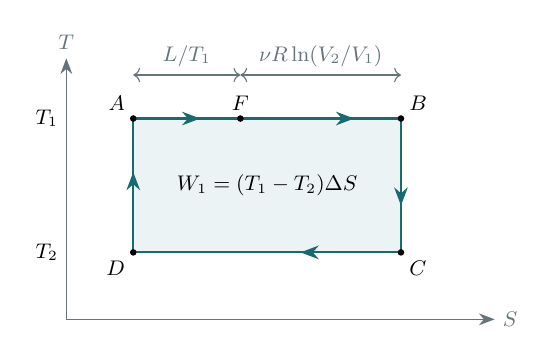
\begin{tikzpicture}[scale=.85,transform shape]

\fill[accent!8] (1,1)--(1,3)--(5,3)--(5,1)--cycle;
\draw[axis] (0,0)--(6.4,0) node[right] {$S$};
\draw[axis] (0,0)--(0,3.9) node[above] {$T$};
\draw[traj] (1,3)--(5,3)--(5,1)--(1,1)--cycle;
\draw[motion] (1.5,3)--(2,3);\draw[motion] (3.4,3)--(4.3,3);
\draw[motion] (5,2.6)--(5,1.7);\draw[motion] (4.4,1)--(3.5,1);
\draw[motion] (1,1.4)--(1,2.2);
\foreach \x/\y/\lab/\pos in {1/3/A/above left,2.6/3/F/above,5/3/B/above right,5/1/C/below right,1/1/D/below left}{\fill (\x,\y) circle (1.4pt) node[\pos] {$\lab$};}
\node[left] at (0,3) {$T_1$};\node[left] at (0,1) {$T_2$};
\draw[axis,<->] (1,3.65)--(2.6,3.65) node[midway,above] {$L/T_1$};
\draw[axis,<->] (2.6,3.65)--(5,3.65) node[midway,above] {$\nu R\ln(V_2/V_1)$};
\node at (3,2) {$W_1=(T_1-T_2)\Delta S$};

\end{tikzpicture}
\figcaption{解图热试2.2C\quad 熵宽含汽化与气相膨胀两部分，围成面积即第一轮功。}
\end{minipage}\end{center}
在所画的例子中，低温压缩先沿气相等温线$CG$减小体积，再在饱和压强下沿$GD$凝结一部分气体。由$S_D=S_A$选择停止凝结的位置，再绝热压缩升温返回$A$。饱和熵、液相比热和状态方程共同决定等熵线落在气相区、两相区或液相区；图B选择与这一闭合关系相容的一种定性情形。气相绝热段$BC$若有常量$\gamma$，还满足$T_1V_2^{\gamma-1}=T_2V_C^{\gamma-1}$，因此$V_C>V_2$，与图中向右下的膨胀方向相同。

解图热试2.2C中$AFB$在$T_1$水平线上，$CD$在$T_2$水平线上，两条绝热线竖直。高温等温边的总熵宽为
\[
\Delta S=\frac{L}{T_1}+\nu R\ln\frac{V_2}{V_1}.
\]
因此低温放热量$Q_c^{(1)}=T_2\Delta S$，第一轮净功等于矩形面积：
\[
\boxed{W_1=(T_1-T_2)\Delta S
=\left(1-\frac{T_2}{T_1}\right)
\left(L+\nu RT_1\ln\frac{V_2}{V_1}\right)}.
\]
求功所需的低温放热量由$T_2\Delta S$直接给出，凝结份额则在给出具体物性后按等熵终点求取。工质的饱和曲线、液相比热等数据未给出，$p$--$V$图只能定性画一种满足熵闭合条件的情形；$T$--$S$图及第一轮功则由可逆性和总吸热确定。
沿$AF$的熵增为$L/T_1$，沿$FB$的熵增为$\nu R\ln(V_2/V_1)$，两部分在图C的高温边上相接。沿$BC$的温度降低而熵保持不变；沿$CD$的温度固定而熵减少同样的$\Delta S$；沿$DA$熵保持不变而温度升高。这四段变化使工质恢复最初的温度、熵和物态，输出功就是吸热与放热之差。随着后续循环推进，热、冷物体温度逐步改变，每轮都在该轮的两端温度间工作，累计后才得到第一问的最大功。



\Needspace{13\baselineskip}

\pdfbookmark[2]{第 3 题 从活塞与分子碰撞导出绝热方程}{q3}

\section*{第 3 题\quad 从活塞与分子碰撞导出绝热方程}\label{q:3}


理想气体封闭在柱形绝热气缸中，一端为密封、无摩擦的刚性活塞。将活塞缓慢推入气缸，分子与活塞作弹性碰撞，获得的能量经分子碰撞重新分配到各自由度。
利用这一微观模型导出气体准静态绝热过程的$T$--$V$关系，设摩尔热容量$C_V$及$\gamma=C_p/C_V$为常量。须给出碰撞通量、单分子能量变化和速度分布积分，并说明“缓慢”怎样进入近似。


\begin{center}\begin{minipage}{.98\linewidth}\centering
\begin{tikzpicture}[scale=.9,transform shape]

\draw[object] (0,2.2)--(0,0)--(5.5,0);
\draw[object] (0,2.2)--(5.5,2.2);
\fill[accent!7] (.03,.03) rectangle (4.5,2.17);
\draw[object,line width=2pt] (4.5,0)--(4.5,2.2);
\draw[object] (4.5,1.1)--(6,1.1);
\draw[motion] (5.7,1.6)--(4.7,1.6) node[midway,above] {$-u\hat x$};
\fill (2.6,1.4) circle (2pt);
\draw[motion] (2.6,1.4)--(3.7,1.4) node[midway,above] {$v_x$};
\draw[axis] (0,-.45)--(6,-.45) node[right] {$x$};
\node at (2, .6) {$n,\ T,\ m$};
\node[above] at (2.3,2.35) {绝热壁};

\end{tikzpicture}
\figcaption{图热试2.3\quad 活塞在右端向左推进，气体分子朝右迎撞。}
\end{minipage}\end{center}

\Needspace{6\baselineskip}\subsection*{解答}


图热试2.3把活塞设在右端，$x$轴向右。活塞以速度$-u\hat x$缓慢向左推进，$u>0$，截面积为$A$，气体体积变化为
\[
\mathrm dV=-Au\,\mathrm dt.
\]
气体在各瞬间近似处于均匀平衡态，数密度$n=N/V$，单分子的$x$速度分量为$v_x$，分布为
\[
f(v_x)=\sqrt{\frac{m}{2\pi kT}}\exp\left(-\frac{mv_x^2}{2kT}\right),
\qquad
\int_{-\infty}^{\infty}f(v_x)\,\mathrm dv_x=1.
\]
分子数密度$n$把单位体积的分子数与速度分布相连，$f(v_x)\mathrm dv_x$是在给定法向速度区间的分子比例。靠近活塞、速度为$v_x$的分子，在$\mathrm dt$内与活塞的相对接近距离为$(v_x+u)\mathrm dt$，这段厚度乘截面积$A$给迎撞分子所占的柱形体积。活塞瞬时系中，入射分子的法向相对速度为$v_x+u$。只有$v_x>-u$的分子能够迎上活塞，单位时间、给定速度区间的碰撞数为
\[
\boxed{\mathrm d\dot N=nA(v_x+u)f(v_x)\,\mathrm dv_x,\qquad v_x>-u}.
\]
\begin{center}\begin{minipage}{.98\linewidth}\centering
\begin{tikzpicture}[scale=.85,transform shape]

\node at (1.5,3.3) {气缸系};
\draw[object,line width=2pt] (3.3,1.4)--(3.3,2.8);
\draw[motion] (.2,2.5)--(2,2.5) node[midway,above] {$v_x$};
\draw[motion] (2,1.7)--(.2,1.7) node[midway,below] {$-v_x-2u$};
\draw[motion] (4.3,2.2)--(3.5,2.2) node[midway,above] {$-u$};
\node at (1.5,.7) {活塞瞬时系};
\draw[object,line width=2pt] (3.3,-1.2)--(3.3,.2);
\draw[motion] (.2,-.1)--(2,-.1) node[midway,above] {$v_x+u$};
\draw[motion] (2,-.9)--(.2,-.9) node[midway,below] {$-(v_x+u)$};
\node[right] at (3.7,-.5) {壁面瞬时静止};

\end{tikzpicture}
\figcaption{解图热试2.3A\quad 壁面系弹性反射后反向，再变回气缸系求能量增量。}
\end{minipage}\end{center}
解图热试2.3A在活塞瞬时系把相对速度反向，再变回气缸系：
\[
v'_x+u=-(v_x+u),\qquad
\boxed{v'_x=-v_x-2u}.
\]
这里先把活塞速度$-u$减去，入射相对速度变为$v_x+u$；弹性反射给相对速度$-(v_x+u)$，再加回$-u$便得到碰后负向速度。若$v_x>0$，碰后速率比碰前增加$2u$。平行活塞面的两个速度分量不变。因此单分子能量增量为
\[
\Delta\varepsilon=\frac m2[(v_x+2u)^2-v_x^2]
=2mu(v_x+u).
\]
计算功率时，将单次能量增量乘以每秒迎撞活塞的分子数，得到传给气体的功率
\[
\boxed{\dot U_{\rm coll}
=2mnAu\int_{-u}^{\infty}(v_x+u)^2 f(v_x)\,\mathrm dv_x}.
\]

入射区间也包括$-u<v_x<0$：这些分子本来已向左运动，但比活塞慢，会被活塞追上。对所有$v_x>-u$，$v_x+u>0$；压入时$u>0$，单次能量增加与总功率都为正。把通量和能增相乘后相对速度平方出现，近零速区间的贡献便由这个权重自然确定。

令热运动速度尺度$s=\sqrt{kT/m}$。准静态要求$u/s\ll1$，并且气体内部的能量再分配、压强均匀化比压缩变化快。对上式整体按$u/s$展开，最低非零阶为
\[
\dot U_{\rm coll}
=2mnAu\int_0^\infty v_x^2f(v_x)\,\mathrm dv_x+O(u^2).
\]
分布在$v_x=0$附近仍有分子；对相对速度平方加权的整个积分作展开后，它们与积分下限移动的影响一起进入较高阶修正。
\begin{center}\begin{minipage}{.98\linewidth}\centering
\begin{tikzpicture}[scale=.85,transform shape]

\draw[axis] (-3.5,0)--(3.7,0) node[right] {$v_x/s$};
\draw[axis] (0,0)--(0,3.4) node[above] {$s f(v_x)$};
\fill[accent!10,domain=0:3,samples=70] (0,0)--plot (\x,{3*exp(-\x*\x/2)})--(3,0)--cycle;
\draw[traj,domain=-3:3,samples=90] plot (\x,{3*exp(-\x*\x/2)});
\draw[guide] (-.3,0)--(-.3,2.87);
\node[below left] at (-.3,0) {$-u/s$};
\node[below right] at (0,0) {$0$};
\node[right] at (1.1,2.5) {主项取正半轴};
\node at (0,-.9) {$\int_0^\infty v_x^2f(v_x)\,\mathrm dv_x=kT/(2m)$};

\end{tikzpicture}
\figcaption{解图热试2.3B\quad 慢活塞极限在积分层面展开，零速附近分子仍存在。}
\end{minipage}\end{center}
解图热试2.3B的高斯分布关于$v_x=0$对称，积分只取正半轴。令$y=v_x/s$，则
\[
\int_0^\infty v_x^2f(v_x)\,\mathrm dv_x
=\frac{s^2}{\sqrt{2\pi}}\int_0^\infty y^2e^{-y^2/2}\,\mathrm dy.
\]
分部积分有
\[
\int_0^\infty y^2e^{-y^2/2}\,\mathrm dy
=\left[-ye^{-y^2/2}\right]_0^\infty
+\int_0^\infty e^{-y^2/2}\,\mathrm dy
=\sqrt{\frac\pi2}.
\]
因此
\[
\int_0^\infty v_x^2f(v_x)\,\mathrm dv_x
=\frac{s^2}{2}=\frac{kT}{2m},
\qquad
\dot U_{\rm coll}=nAkTu+O(u^2).
\]
\begin{center}\begin{minipage}{.98\linewidth}\centering
\begin{tikzpicture}[scale=.8,transform shape]
\draw[axis] (0,0)--(10.7,0) node[right] {$a=u/s$};
\draw[axis] (0,0)--(0,3.2) node[above] {$\dot U/(nAkTu)$};
\node[above] at (5,3.5) {固定瞬时Maxwell分布，零速处取连续极限1};
\draw[traj] plot coordinates {(0.000000000,0.757208171) (0.083333333,0.766471777) (0.166666667,0.775827927) (0.250000000,0.785277277) (0.333333333,0.794820487) (0.416666667,0.804458217) (0.500000000,0.814191129) (0.583333333,0.824019888) (0.666666667,0.833945159) (0.750000000,0.843967609) (0.833333333,0.854087906) (0.916666667,0.864306722) (1.000000000,0.874624726) (1.083333333,0.885042594) (1.166666667,0.895560998) (1.250000000,0.906180616) (1.333333333,0.916902123) (1.416666667,0.927726200) (1.500000000,0.938653526) (1.583333333,0.949684783) (1.666666667,0.960820653) (1.750000000,0.972061819) (1.833333333,0.983408967) (1.916666667,0.994862784) (2.000000000,1.006423956) (2.083333333,1.018093172) (2.166666667,1.029871123) (2.250000000,1.041758497) (2.333333333,1.053755988) (2.416666667,1.065864288) (2.500000000,1.078084090) (2.583333333,1.090416090) (2.666666667,1.102860983) (2.750000000,1.115419466) (2.833333333,1.128092236) (2.916666667,1.140879991) (3.000000000,1.153783431) (3.083333333,1.166803255) (3.166666667,1.179940163) (3.250000000,1.193194858) (3.333333333,1.206568041) (3.416666667,1.220060414) (3.500000000,1.233672682) (3.583333333,1.247405547) (3.666666667,1.261259714) (3.750000000,1.275235889) (3.833333333,1.289334776) (3.916666667,1.303557082) (4.000000000,1.317903512) (4.083333333,1.332374775) (4.166666667,1.346971576) (4.250000000,1.361694623) (4.333333333,1.376544625) (4.416666667,1.391522288) (4.500000000,1.406628322) (4.583333333,1.421863436) (4.666666667,1.437228337) (4.750000000,1.452723735) (4.833333333,1.468350339) (4.916666667,1.484108857) (5.000000000,1.500000000) (5.083333333,1.516024476) (5.166666667,1.532182995) (5.250000000,1.548476265) (5.333333333,1.564904996) (5.416666667,1.581469898) (5.500000000,1.598171678) (5.583333333,1.615011045) (5.666666667,1.631988709) (5.750000000,1.649105377) (5.833333333,1.666361758) (5.916666667,1.683758559) (6.000000000,1.701296488) (6.083333333,1.718976252) (6.166666667,1.736798557) (6.250000000,1.754764111) (6.333333333,1.772873619) (6.416666667,1.791127786) (6.500000000,1.809527318) (6.583333333,1.828072919) (6.666666667,1.846765292) (6.750000000,1.865605142) (6.833333333,1.884593170) (6.916666667,1.903730078) (7.000000000,1.923016569) (7.083333333,1.942453342) (7.166666667,1.962041097) (7.250000000,1.981780534) (7.333333333,2.001672350) (7.416666667,2.021717243) (7.500000000,2.041915910) (7.583333333,2.062269046) (7.666666667,2.082777346) (7.750000000,2.103441503) (7.833333333,2.124262211) (7.916666667,2.145240161) (8.000000000,2.166376044) (8.083333333,2.187670549) (8.166666667,2.209124366) (8.250000000,2.230738181) (8.333333333,2.252512681) (8.416666667,2.274448550) (8.500000000,2.296546474) (8.583333333,2.318807133) (8.666666667,2.341231210) (8.750000000,2.363819384) (8.833333333,2.386572335) (8.916666667,2.409490740) (9.000000000,2.432575274) (9.083333333,2.455826612) (9.166666667,2.479245427) (9.250000000,2.502832391) (9.333333333,2.526588174) (9.416666667,2.550513445) (9.500000000,2.574608871) (9.583333333,2.598875116) (9.666666667,2.623312846) (9.750000000,2.647922723) (9.833333333,2.672705406) (9.916666667,2.697661556) (10.000000000,2.722791829)};
\node[below] at (0,-.12) {$-0.4$};
\node[below] at (5,-.12) {$0$};
\node[below] at (10,-.12) {$0.4$};
\end{tikzpicture}
\figcaption{解图热试2.3D\quad 固定瞬时Maxwell分布，零速处取连续极限1}
\end{minipage}\end{center}
图D以$a=u/s$表示活塞速度，把完整瞬时积分除以$nAkTu$，零速处取连续极限。纵坐标可写为$2\int_{-a}^{\infty}(y+a)^2e^{-y^2/2}\mathrm dy/\sqrt{2\pi}$；在$a=0$它等于1，压入时为大于1的修正，外移时为小于1的修正。这里比较同一瞬时平衡分布下的壁面响应，气体全过程保持近似平衡还依赖内部碰撞和压强传播的时间尺度。

半轴二阶矩还可与三维速率分布相连：令$F(v)=4\pi[m/(2\pi kT)]^{3/2}v^2e^{-mv^2/(2kT)}$，则在$v>0$有$v^2f(v)=[kT/(2m)]F(v)$。由$\int_0^\infty F(v)\,\mathrm dv=1$，直接得到同一半轴积分$kT/(2m)$。这里$f$是单个速度分量的分布，$F$包含三维速度空间球壳的因子$4\pi v^2$。

保留准静态主项并用$\mathrm dV=-Au\,\mathrm dt$，得到
\[
\boxed{\mathrm dU=-nkT\,\mathrm dV}.
\]
这里的能量增量由活塞碰撞逐次累加得到，接着用气体内能与温度的关系计算温升。再利用气体平衡态的内能关系与$N=\nu N_A$：
\[
\nu C_V\,\mathrm dT=-\frac NVkT\,\mathrm dV
=-\nu RT\frac{\mathrm dV}{V}.
\]
分子与壁面碰撞直接改变法向平动能，分子间相互碰撞再把能量分配到其余平动、转动等有效自由度，所以此处的$C_V$是气体的全部摩尔热容量。用$C_V=R/(\gamma-1)$，整理为
\[
\frac{\mathrm dT}{T}+(\gamma-1)\frac{\mathrm dV}{V}=0.
\]
积分得
\[
\boxed{TV^{\gamma-1}=\text{常量}}.
\]
\begin{center}\begin{minipage}{.98\linewidth}\centering
\begin{tikzpicture}[scale=.85,transform shape]

\draw[axis] (0,0)--(5.3,0) node[right] {$V$};
\draw[axis] (0,0)--(0,3.8) node[above] {$T$};
\draw[traj,domain=1:4.5,samples=70] plot (\x,{3.2/\x^.6666667});
\draw[motion] (3,1.538)--(2.5,1.737);
\node[above right] at (1,3.2) {压缩升温};
\node at (3.2,3) {$TV^{\gamma-1}=\text{常量}$};
\node at (3.3,2.45) {示意：$\gamma=5/3$};

\end{tikzpicture}
\figcaption{解图热试2.3C\quad 准静态绝热压缩轨迹向左上方移动。}
\end{minipage}\end{center}
解图热试2.3C中活塞压入使$V$减小、$T$升高，轨迹在$T$--$V$平面向左上方走。与$pV=\nu RT$合用还得$pV^\gamma=\text{常量}$。增大活塞推进速度时，碰撞积分保留较高阶项，气体还可能出现非均匀流动与非平衡分布；此时按分布演化计算壁面传能和状态变化。
从初态$(T_i,V_i)$积分到任意准静态中间态时，$\ln(T/T_i)=-(\gamma-1)\ln(V/V_i)$。压缩有$V/V_i<1$，右侧为正，故$T>T_i$；膨胀则相反。与状态方程联用得到压强沿$p\propto V^{-\gamma}$增加，图C的温度路径与这一压强变化由同一能量输入决定。缓慢条件还要求一次显著体积变化所需的时间远长于分子碰撞弛豫与声传播时间，这样每一步才能继续使用均匀温度和同一Maxwell分布。



\Needspace{13\baselineskip}

\pdfbookmark[2]{第 4 题 导热稳态、分子扩散与撤热源后的平衡}{q4}

\section*{第 4 题\quad 导热稳态、分子扩散与撤热源后的平衡}\label{q:4}


侧面绝热的柱形容器由长度$L$的均匀固体分隔成等体积区域1、2，两区装相同分子的理想气体，区域1的气体质量为区域2的两倍。固体不能移动，热膨胀忽略，导热系数与横截面积均为常量。两区分别由温度$T_1$与$T_2>T_1$的热源维持温度，忽略各气区内部温差，已达到导热稳态。
\begin{enumerate}
\item 求固体沿轴向的温度分布，取左端$x=0$、右端$x=L$。
\item 同时跟踪两区各一个分子，时间$t$远长于平均碰撞间隔，但跟踪期间未遇容器壁。求其离初始点的典型距离之比，以均方根位移$R_{i,\rm rms}=\sqrt{\langle|\boldsymbol R_i|^2\rangle}$表示；并说明这个统计比值与单次轨迹距离比的关系。
\item 定体摩尔热容量$C_V$为常量，区域2有$\nu_2$ mol气体。固体有$\nu_s$ mol、摩尔热容量$C_s$，满足$\nu_sC_s=2\nu_2C_V$。撤去两热源，使整体与外界绝热，求最终共同温度。
\end{enumerate}
第（2）问采用各向同性随机飞行近似：相邻自由程方向独立、长度服从均值$\lambda$的指数分布，平均速率$\bar v\propto\sqrt T$，相同硬球分子的$\lambda\propto1/n$。


\begin{center}\begin{minipage}{.98\linewidth}\centering
\begin{tikzpicture}[scale=.9,transform shape]

\draw[object] (0,0) rectangle (7,2.2);
\fill[accent!8] (.03,.03) rectangle (2.3,2.17);
\fill[muted!12] (2.3,.03) rectangle (4.7,2.17);
\fill[warm!8] (4.7,.03) rectangle (6.97,2.17);
\draw[object] (2.3,0)--(2.3,2.2);\draw[object] (4.7,0)--(4.7,2.2);
\node[align=center] at (1.15,1.1) {区域1\\$T_1,\ 2\nu_2$};
\node[align=center] at (3.5,1.1) {固体\\$\nu_sC_s$};
\node[align=center] at (5.85,1.1) {区域2\\$T_2,\ \nu_2$};
\draw[axis] (2.3,-.6)--(5.2,-.6) node[right] {$x$};
\node[below] at (2.3,-.6) {$0$};\node[below] at (4.7,-.6) {$L$};
\node[above] at (3.5,2.4) {侧面绝热；$T_2>T_1$};

\end{tikzpicture}
\figcaption{图热试2.4\quad 两气区体积相等，固体温度由左右热源维持。}
\end{minipage}\end{center}

\Needspace{6\baselineskip}\subsection*{解答}


图热试2.4规定$x$由冷侧1指向热侧2。稳态时固体内部不蓄热，任一横截面的导热功率相同，傅里叶定律给
\[
\dot Q_x=-kA\frac{\mathrm dT_s}{\mathrm dx}=\text{常量}.
\]
取固体的任意薄层，稳态下薄层内部能量随时间保持，所以流入热量等于流出热量，导热功率沿$x$不变。$k,A$均恒定，故$\mathrm dT_s/\mathrm dx$为常量。用两端的指定温度$T_s(0)=T_1,T_s(L)=T_2$，
\[
\boxed{T_s(x)=T_1+\frac{T_2-T_1}{L}x},\qquad
\dot Q_x=-\frac{kA}{L}(T_2-T_1)<0.
\]
\begin{center}\begin{minipage}{.98\linewidth}\centering
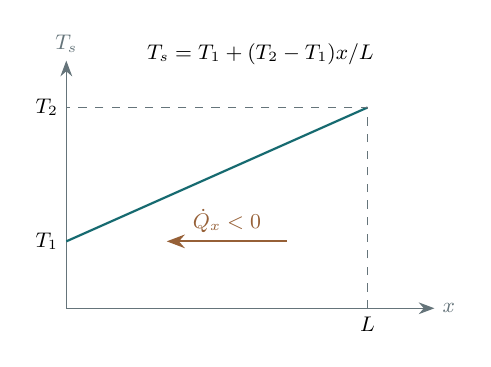
\begin{tikzpicture}[scale=.85,transform shape]

\draw[axis] (0,0)--(5.5,0) node[right] {$x$};
\draw[axis] (0,0)--(0,3.7) node[above] {$T_s$};
\draw[traj] (0,1)--(4.5,3);
\draw[guide] (4.5,0)--(4.5,3)--(0,3);
\node[left] at (0,1) {$T_1$};\node[left] at (0,3) {$T_2$};
\node[below] at (4.5,0) {$L$};
\draw[force] (3.3,1)--(1.5,1) node[midway,above] {$\dot Q_x<0$};
\node at (2.9,3.8) {$T_s=T_1+(T_2-T_1)x/L$};

\end{tikzpicture}
\figcaption{解图热试2.4A\quad 稳态温度梯度向右，热流由右向左。}
\end{minipage}\end{center}
解图热试2.4A中温度直线向右升高，热流箭头却向左，二者方向相反；稳态导热中各处温度随时间保持，同时热量持续从右端热源传向左端热源。

第（2）问把一次自由程向量记为$\boldsymbol\ell_j$。分子经过$M$段后
\[
\boldsymbol R=\sum_{j=1}^M\boldsymbol\ell_j,\qquad
\langle R^2\rangle
=\sum_j\langle\ell_j^2\rangle+
2\sum_{i<j}\langle\boldsymbol\ell_i\cdot\boldsymbol\ell_j\rangle.
\]
各段方向独立、各向同性，使不同段的交叉项在统计平均后为零，故
\[
\langle R^2\rangle=M\langle\ell^2\rangle.
\]
按给定指数分布，
\[
\langle\ell^2\rangle
=\int_0^\infty\ell^2\frac{e^{-\ell/\lambda}}{\lambda}\,\mathrm d\ell
=\lambda^2\int_0^\infty y^2e^{-y}\,\mathrm dy
=2\lambda^2.
\]
积分中的$\int_0^\infty y^2e^{-y}\mathrm dy$分部积分两次，依次化为$2\int_0^\infty ye^{-y}\mathrm dy=2\int_0^\infty e^{-y}\mathrm dy=2$；指数分布的长自由程尾部因此使二阶矩等于均值平方的2倍。长时间平均碰撞段数$M\simeq\bar vt/\lambda$，所以
\[
\boxed{R_{\rm rms}\simeq\sqrt{2\bar v\lambda t}}.
\]
\begin{center}\begin{minipage}{.98\linewidth}\centering
\begin{tikzpicture}[scale=.75,transform shape]

\draw[object] (0,0)--(.8,.45)--(.3,1.2)--(1.2,1.5)--(1.9,.9)--(1.5,.2)--(2.4,-.2)--(3,.6)--(2.8,1.3)--(3.6,1.7);
\fill (0,0) circle (1.7pt) node[below left] {$O$};
\fill (3.6,1.7) circle (1.7pt) node[above] {$P$};
\draw[motion] (0,0)--(3.6,1.7) node[midway,below right] {$\boldsymbol R$};
\draw[axis,<->] (.15,1.45)--(1.05,1.75) node[midway,above] {$\boldsymbol\ell_j$};
\node[right,align=left] at (4.4,1.2) {$\langle\boldsymbol\ell_i\cdot\boldsymbol\ell_j\rangle=0$\\[7pt]$\langle\ell^2\rangle=2\lambda^2$\\[7pt]$\langle R^2\rangle\simeq2\bar v\lambda t$};
\node at (3.5,-1) {折线路程与端到端位移不同};

\end{tikzpicture}
\figcaption{解图热试2.4B\quad 随机飞行的统计平均消去交叉项，单条轨迹仍会波动。}
\end{minipage}\end{center}
解图热试2.4B画同一模型中的折线轨迹与端到端位移；折线路程约为$\bar vt$，端到端位移只按$\sqrt t$增长。等体积、相同分子且质量比为2给$n_1=2n_2$，于是
\[
\frac{\lambda_1}{\lambda_2}=\frac12,\qquad
\frac{\bar v_1}{\bar v_2}=\sqrt{\frac{T_1}{T_2}},
\]
\[
\boxed{\frac{R_{1,\rm rms}}{R_{2,\rm rms}}
=\frac1{\sqrt2}\left(\frac{T_1}{T_2}\right)^{1/4}}.
\]
相同分子的平均速率为$\bar v=\sqrt{8k_BT/(\pi m)}$，硬球模型的平均自由程为$\lambda=1/(\sqrt2\pi d^2n)$，其中$d$为分子有效直径。用压强也能表达相同的密度信息：$p_1V=2\nu_2RT_1$、$p_2V=\nu_2RT_2$，所以$p_2/p_1=T_2/(2T_1)$。硬球自由程$\lambda=k_BT/(\sqrt2\pi d^2p)$给$R_{\rm rms}\propto T^{3/4}p^{-1/2}$，代入此压强比仍得上述四分之一次方结果。固体固定使两气区保持各自体积，压强由各自粒子数和温度确定。

这个比值描述许多轨迹的统计尺度。单条轨迹的交叉项随随机方向涨落，单个分子的位移也随之波动；取大量同条件轨迹的均方根后得到所求比值。

若定义扩散系数$D=\bar v\lambda/3$，则$\langle R^2\rangle=6Dt$，每一坐标的方差为$2Dt$。典型观察窗口既要满足$t\gg\lambda/\bar v$以积累许多次碰撞，也要使$R_{\rm rms}$小于到容器壁的距离，以保持所用自由空间随机飞行近似。这里统计的是位移平方的平均，路线长度则是许多自由程长度之和。

第（3）问中$\nu_1=2\nu_2$。固体初态有线性温度分布，等体积薄片的热容量均匀，所以其初始热能对应的平均温度为
\[
\bar T_{s0}=\frac1L\int_0^L T_s(x)\,\mathrm dx
=\frac{T_1+T_2}{2}.
\]
\begin{center}\begin{minipage}{.98\linewidth}\centering
\begin{tikzpicture}[scale=.85,transform shape]

\draw[guide,rounded corners] (-.3,-.4) rectangle (7.3,2.5);
\draw[object,fill=accent!8] (0,0) rectangle (2,2);
\draw[object,fill=muted!10] (2.5,0) rectangle (4.5,2);
\draw[object,fill=warm!8] (5,0) rectangle (7,2);
\node[align=center] at (1,1) {气区1\\$2K,\ T_1$};
\node[align=center] at (3.5,1) {固体\\$2K,\ \bar T_{s0}$};
\node[align=center] at (6,1) {气区2\\$K,\ T_2$};
\node[above] at (3.5,2.7) {$\bar T_{s0}=(T_1+T_2)/2$};
\node at (3.5,-1) {撤热源，整体绝热，最终各处同温 $T_f$};

\end{tikzpicture}
\figcaption{解图热试2.4C\quad 三个热容量权重与固体初始平均能量决定终温。}
\end{minipage}\end{center}
解图热试2.4C把三个热容量分别标为$2K,K,2K$，其中$K=\nu_2C_V$。撤热源后无外界热量、无体积功，能量守恒为
\[
2K(T_f-T_1)+K(T_f-T_2)
+\frac{2K}{L}\int_0^L[T_f-T_s(x)]\,\mathrm dx=0.
\]
固体每个厚度$\mathrm dx$的薄片具有热容量$2K\mathrm dx/L$，其最终能量变化为该热容量乘$T_f-T_s(x)$。把左右两气区与所有薄片的带符号能量变化相加，即得上式；刚性容器与固定隔体保持体积，所以所用气体热容量是定体热容量。积分得
\[
2(T_f-T_1)+(T_f-T_2)+2T_f-T_1-T_2=0,
\]
\[
\boxed{T_f=\frac{3T_1+2T_2}{5}}.
\]
该温度位于$T_1,T_2$之间。固体初始冷端会升温、热端会降温，整个固体的净吸放热取决于它与$T_f$的平均温差，每个薄片按自己的初温与最终温度之差计入代数热量。\begin{center}\begin{minipage}{.98\linewidth}\centering
\begin{tikzpicture}[scale=.8,transform shape]
\draw[axis] (0,0)--(10.7,0) node[right] {$x/L$};
\draw[axis] (0,0)--(0,3.2) node[above] {$(T_f-T_s)/\Delta T$};
\node[above] at (5,3.5) {冷端部分最终升温，热端部分最终降温};
\draw[traj] plot coordinates {(0.000000000,3.000000000) (0.083333333,2.975000000) (0.166666667,2.950000000) (0.250000000,2.925000000) (0.333333333,2.900000000) (0.416666667,2.875000000) (0.500000000,2.850000000) (0.583333333,2.825000000) (0.666666667,2.800000000) (0.750000000,2.775000000) (0.833333333,2.750000000) (0.916666667,2.725000000) (1.000000000,2.700000000) (1.083333333,2.675000000) (1.166666667,2.650000000) (1.250000000,2.625000000) (1.333333333,2.600000000) (1.416666667,2.575000000) (1.500000000,2.550000000) (1.583333333,2.525000000) (1.666666667,2.500000000) (1.750000000,2.475000000) (1.833333333,2.450000000) (1.916666667,2.425000000) (2.000000000,2.400000000) (2.083333333,2.375000000) (2.166666667,2.350000000) (2.250000000,2.325000000) (2.333333333,2.300000000) (2.416666667,2.275000000) (2.500000000,2.250000000) (2.583333333,2.225000000) (2.666666667,2.200000000) (2.750000000,2.175000000) (2.833333333,2.150000000) (2.916666667,2.125000000) (3.000000000,2.100000000) (3.083333333,2.075000000) (3.166666667,2.050000000) (3.250000000,2.025000000) (3.333333333,2.000000000) (3.416666667,1.975000000) (3.500000000,1.950000000) (3.583333333,1.925000000) (3.666666667,1.900000000) (3.750000000,1.875000000) (3.833333333,1.850000000) (3.916666667,1.825000000) (4.000000000,1.800000000) (4.083333333,1.775000000) (4.166666667,1.750000000) (4.250000000,1.725000000) (4.333333333,1.700000000) (4.416666667,1.675000000) (4.500000000,1.650000000) (4.583333333,1.625000000) (4.666666667,1.600000000) (4.750000000,1.575000000) (4.833333333,1.550000000) (4.916666667,1.525000000) (5.000000000,1.500000000) (5.083333333,1.475000000) (5.166666667,1.450000000) (5.250000000,1.425000000) (5.333333333,1.400000000) (5.416666667,1.375000000) (5.500000000,1.350000000) (5.583333333,1.325000000) (5.666666667,1.300000000) (5.750000000,1.275000000) (5.833333333,1.250000000) (5.916666667,1.225000000) (6.000000000,1.200000000) (6.083333333,1.175000000) (6.166666667,1.150000000) (6.250000000,1.125000000) (6.333333333,1.100000000) (6.416666667,1.075000000) (6.500000000,1.050000000) (6.583333333,1.025000000) (6.666666667,1.000000000) (6.750000000,0.975000000) (6.833333333,0.950000000) (6.916666667,0.925000000) (7.000000000,0.900000000) (7.083333333,0.875000000) (7.166666667,0.850000000) (7.250000000,0.825000000) (7.333333333,0.800000000) (7.416666667,0.775000000) (7.500000000,0.750000000) (7.583333333,0.725000000) (7.666666667,0.700000000) (7.750000000,0.675000000) (7.833333333,0.650000000) (7.916666667,0.625000000) (8.000000000,0.600000000) (8.083333333,0.575000000) (8.166666667,0.550000000) (8.250000000,0.525000000) (8.333333333,0.500000000) (8.416666667,0.475000000) (8.500000000,0.450000000) (8.583333333,0.425000000) (8.666666667,0.400000000) (8.750000000,0.375000000) (8.833333333,0.350000000) (8.916666667,0.325000000) (9.000000000,0.300000000) (9.083333333,0.275000000) (9.166666667,0.250000000) (9.250000000,0.225000000) (9.333333333,0.200000000) (9.416666667,0.175000000) (9.500000000,0.150000000) (9.583333333,0.125000000) (9.666666667,0.100000000) (9.750000000,0.075000000) (9.833333333,0.050000000) (9.916666667,0.025000000) (10.000000000,0.000000000)};
\node[below] at (0,-.12) {$0$};
\node[below] at (4,-.12) {$2/5$};
\node[below] at (10,-.12) {$1$};
\draw[guide] (0,1.8)--(10,1.8) node[right] {$0$};\node[left] at (0,0) {$-3/5$};\node[left] at (0,3) {$2/5$};\end{tikzpicture}
\figcaption{解图热试2.4D\quad 冷端部分最终升温，热端部分最终降温}
\end{minipage}\end{center}
图D用$\Delta T=T_2-T_1$表示固体局部的最终温差：$[T_f-T_s(x)]/\Delta T=2/5-x/L$。在$x=2L/5$处变号，冷端的$2L/5$长度最终升温，其余部分最终降温。固体净热量为$-K\Delta T/5$，区域1吸热$4K\Delta T/5$，区域2放热$3K\Delta T/5$，三者的代数和为零。温度场初态的不均匀与终态的共同温度在这个薄片积分中连续衔接。



\Needspace{13\baselineskip}

\pdfbookmark[2]{第 5 题 光子气体的压强、绝热关系与辐射能流}{q5}

\section*{第 5 题\quad 光子气体的压强、绝热关系与辐射能流}\label{q:5}


黑体空腔的热辐射视为光子气体。频率为$\nu$的光子能量$\varepsilon=h\nu$、动量大小$p_\gamma=h\nu/c$；按频段记数密度$n_\nu$、能量密度$u_\nu=n_\nu h\nu$，总能量密度$u=\sum_\nu u_\nu$。光子静质量为零。热平衡时速度大小均为$c$，方向各向同性。
\begin{enumerate}
\item 先将壁面视为理想反射面，证明辐射压强$p=u/3$。
\item 对充分热化的黑体辐射，结合热力学第二定律说明$u$与壁材、腔体体积无关，只依赖温度，并导出$u=aT^4$。采用忽略表面与有限尺寸效应的宏观腔体近似。
\item 导出准静态可逆绝热过程中$p$与体积$V$的关系。
\item 求任意一光子的$x$方向速度分量分布$f(v_x)$。
\item 在壁上开一个不扰动内部平衡的小孔，证明单位孔面积的向外辐射功率$J=cu/4$，由此给出$J$随温度的规律。
\end{enumerate}
可用热力学恒等式
\[
\left(\frac{\partial U}{\partial V}\right)_T
=T\left(\frac{\partial p}{\partial T}\right)_V-p.
\]
空腔在求平衡态时允许吸收、发射以充分热化；反射面用于计算瞬时动量传递和理想绝热过程。


\begin{center}\begin{minipage}{.98\linewidth}\centering
\begin{tikzpicture}[scale=.9,transform shape]

\draw[object,fill=accent!4] (0,0) rectangle (6,3.6);
\draw[motion] (1,2.6)--(6,.8);
\draw[motion] (6,.8)--(3.77777778,0);
\draw[motion] (4.4,2.9)--(5.8,2.1);
\draw[motion] (1.1,.5)--(.15,1.8);
\draw[axis] (6,1.8)--(7.5,1.8) node[right] {$+\hat x$};
\node[align=center] at (2.2,3.1) {各向同性热辐射};
\node at (3,-1) {$\varepsilon=h\nu,\quad p_\gamma=\varepsilon/c$};
\node[below] at (3,-.2) {充分热化的宏观空腔};

\end{tikzpicture}
\figcaption{图热试2.5\quad 以腔壁法线定义x方向，光子方向各向同性。}
\end{minipage}\end{center}

\Needspace{6\baselineskip}\subsection*{解答}


图热试2.5取壁面外法线为$+\hat x$。光子静质量为零，动量大小为$\varepsilon/c$，反射受力直接按能量与动量的这一关系计算。
先看频段$\nu$、方向立体角$\mathrm d\Omega$内的一束光，能量密度为$u_\nu\mathrm d\Omega/(4\pi)$，与外法线夹角为$\theta$，只取指向壁面的半球$0\le\theta\le\pi/2$。
\begin{center}\begin{minipage}{.98\linewidth}\centering
\begin{tikzpicture}[scale=.85,transform shape]

\draw[object,line width=2pt] (3,-2.2)--(3,2.2);
\draw[motion] (-.2,1.8)--(3,0) node[pos=.36,above] {入射};
\draw[motion] (3,0)--(-.2,-1.8) node[pos=.7,below] {反射};
\draw[axis] (3,0)--(5.3,0) node[right] {$+\hat x$};
\draw[guide] (3,0)--(4.6,-.9);
\draw (3.85,0) arc[start angle=0,end angle=-29.36,radius=.85];
\node at (4.1,-.31) {$\theta$};
\draw[force] (3.1,.8)--(4.8,.8) node[midway,above] {$\Delta p_x=2\varepsilon\cos\theta/c$};
\node at (1,-2.6) {$\mathrm dJ=(u/4\pi)c\cos\theta\,\mathrm d\Omega$};

\end{tikzpicture}
\figcaption{解图热试2.5A\quad 碰撞通量与反射动量各含一次法向投影。}
\end{minipage}\end{center}
解图热试2.5A中单位面积、单位时间到达壁面的能量为
\[
\mathrm dJ_\nu=\frac{u_\nu}{4\pi}c\cos\theta\,\mathrm d\Omega.
\]
一次反射传给壁面的法向动量为$2(\varepsilon/c)\cos\theta$，所以该束光的压强贡献为
\[
\mathrm dp_\nu=\frac{2\cos\theta}{c}\,\mathrm dJ_\nu
=\frac{2u_\nu}{4\pi}\cos^2\theta\,\mathrm d\Omega.
\]
在光滑反射中，光子传给壁面的切向动量为零，法向动量在反射前后反向，壁面所获法向动量为正。一个$\cos\theta$来自光子在单位时间到达壁面的厚度$c\cos\theta\mathrm dt$，另一个来自单个光子的法向动量。对绕法线的方位角积分给$2\pi$，而朝壁面的极角只取$0$到$\pi/2$。用$\mathrm d\Omega=2\pi\sin\theta\,\mathrm d\theta$积分，
\[
p_\nu=\frac{2u_\nu}{4\pi}
\int_0^{\pi/2}\cos^2\theta\,2\pi\sin\theta\,\mathrm d\theta
=\frac{u_\nu}{3}.
\]
角积分$\int_0^{\pi/2}\cos^2\theta\sin\theta\mathrm d\theta$用$\mu=\cos\theta$换元后为$\int_0^1\mu^2\mathrm d\mu=1/3$。等价地，各向同性使三个方向的动量通量二阶矩相等，方向余弦平方之和为1，每一个方向贡献总能量密度的三分之一。对所有频段相加便得
\[
\boxed{p=\frac13u}.
\]

第（2）问先区分充分热化的黑体辐射与只反射、光子数被人为固定的非热化光场。黑体壁可以吸收、发射光子，平衡光子数随温度与体积调节；固定分子数气体还需指定的粒子密度，在这里由充分热化的平衡条件一同确定。
\begin{center}\begin{minipage}{.98\linewidth}\centering
\begin{tikzpicture}[scale=.75,transform shape]

\draw[object,fill=accent!5] (0,0) rectangle (2.8,2.4);
\draw[object,fill=warm!5] (5.5,0) rectangle (8.3,2.4);
\draw[object] (2.8,.8)--(5.5,.8);\draw[object] (2.8,1.6)--(5.5,1.6);
\draw[object,line width=2pt] (4.1,.8)--(4.1,1.6);
\node[align=center] at (1.4,1.2) {腔1\\壁材1，体积 $V_a$\\同温 $T$};
\node[align=center] at (6.9,1.2) {腔2\\壁材2，体积 $V_b$\\同温 $T$};
\node at (4.1,3.2) {反证假设：$u_1\ne u_2$};
\draw[force] (3,2)--(4,2);\draw[force] (5.2,2)--(4.4,2);
\node[above] at (3.4,2) {$p_1$};\node[above] at (4.9,2) {$p_2$};
\node at (4.1,-.8) {同一温度热库维持热化；活塞取功};

\end{tikzpicture}
\figcaption{解图热试2.5B\quad 同温壁材若能维持辐射压差，就可构造单温度取功矛盾。}
\end{minipage}\end{center}
解图热试2.5B的两个宏观空腔由同一温度热库维持。若仅因壁材不同就有不同的平衡辐射能量密度，由$p=u/3$也会有辐射压差，反射活塞受到相应的净推力。将两腔以小孔连通时，因方向分布相同，双向辐射通量各正比于所在腔的能量密度，净能量由较大$u$的一腔流向较小$u$的一腔。若同温下已有$u_1>u_2$，由温度变化的连续性，可把腔1温度略降至$T_c$、腔2略升至$T_h>T_c$，仍保持$u_1>u_2$，于是热量$Q$可从冷端自行传到热端。再令可逆热机从热端吸取同样的$Q$，向冷端放回$QT_c/T_h$，并输出$W=Q(1-T_c/T_h)>0$。热端恢复原状，光路和热机完成循环，唯一净结果是从冷端单一热库取热$W$并全部变功，违反开尔文表述。因此同温充分热化辐射的能量密度与壁材无关，辐射压强也相同。
体积方面，在忽略边界效应的宏观极限，充分热化辐射是均匀、可加的系统；将同温空腔分成或连成不同体积，不改变各局部的平衡状态。于是
\[
\boxed{u=u(T),\qquad U=u(T)V}.
\]
平衡条件还给出同一结论：光子数不守恒使化学势$\mu_\gamma=0$，均匀系统的欧拉关系为$U=TS-pV$；对欧拉关系直接微分有$\mathrm dU=T\mathrm dS+S\mathrm dT-p\mathrm dV-V\mathrm dp$，与$\mathrm dU=T\,\mathrm dS-p\,\mathrm dV$比较，得$S\,\mathrm dT=V\,\mathrm dp$。同温时$\mathrm dp=0$，压强由共同温度确定，改变宏观体积时保持相同。这里的$U$只计宏观腔内辐射能，腔壁能量另记。

这里的可加性指同温辐射系统的体积和能量同时放大时，能量密度保持不变；忽略表面与有限尺寸影响时，各局部处于同样的热平衡状态。光子数的吸收、发射使平衡态没有额外独立的数密度条件，能量的状态关系采用$U(S,V)$，光子的化学势为零。

将$U=u(T)V$与$p=u/3$代入题给恒等式：
\[
u=T\frac13\frac{\mathrm du}{\mathrm dT}-\frac13u,
\qquad
\frac{\mathrm du}{u}=4\frac{\mathrm dT}{T}.
\]
恒等式左侧的偏导在固定温度下取值，$u(T)$保持不变，所以$\partial U/\partial V=u$；右侧压强对温度的导数为$(1/3)\mathrm du/\mathrm dT$。整理后$T\mathrm du/\mathrm dT=4u$，从$(T_0,u_0)$积分有$\ln(u/u_0)=4\ln(T/T_0)$，正能量密度给正的比例常量$a=u_0/T_0^4$。积分得
\[
\boxed{u=aT^4,\qquad p=\frac a3T^4},
\]
其中$a$为与材料、体积无关的常量，其数值由微观统计或实验确定。

第（3）问在可逆准静态绝热过程中，
\[
\mathrm dU+p\,\mathrm dV=0.
\]
用$U=3pV$展开，
\[
3V\,\mathrm dp+3p\,\mathrm dV+p\,\mathrm dV=0,
\qquad
\frac{\mathrm dp}{p}+\frac43\frac{\mathrm dV}{V}=0.
\]
所以
\[
\boxed{pV^{4/3}=\text{常量}},
\qquad
\boxed{TV^{1/3}=\text{常量}}.
\]
\begin{center}\begin{minipage}{.98\linewidth}\centering
\begin{tikzpicture}[scale=.85,transform shape]

\draw[axis] (0,0)--(5.3,0) node[right] {$V$};
\draw[axis] (0,0)--(0,3.8) node[above] {$p$};
\draw[traj,domain=1:4.5,samples=70] plot (\x,{3.2/\x^1.3333333});
\draw[motion] (2,1.27)--(2.45,.969);
\node at (3.5,3.1) {$pV^{4/3}=\text{常量}$};
\node at (3.5,2.5) {$TV^{1/3}=\text{常量}$};
\node[below] at (2.8,.4) {膨胀降温};

\end{tikzpicture}
\figcaption{解图热试2.5C\quad 辐射可逆绝热膨胀曲线，指数由$U=3pV$决定。}
\end{minipage}\end{center}
进一步用$u=aT^4$写温度方程，$\mathrm dU=4aVT^3\mathrm dT+aT^4\mathrm dV$，第一定律化为$4aVT^3\mathrm dT+(4/3)aT^4\mathrm dV=0$，即$\mathrm dT/T+\mathrm dV/(3V)=0$。这给与压力式相同的温度绝热线。若体积从$V_i$变到$V_f$，总辐射能满足$U_f/U_i=(V_i/V_f)^{1/3}$，输出的体积功为$U_i-U_f$，热量为零。

解图热试2.5C的膨胀方向向右下，温度按$V^{-1/3}$下降。这里平衡光子数通过吸收、发射调节，指数$4/3$直接由辐射状态关系与能量守恒确定；固定物质的量气体的$C_p/C_V$则按粒子数固定的另一组状态约束定义。

第（4）问在速度空间中，所有端点都位于半径$c$的球面上且等概率。解图热试2.5D在$x$方向切取宽度$\mathrm dv_x$的球带。
\begin{center}\begin{minipage}{.98\linewidth}\centering
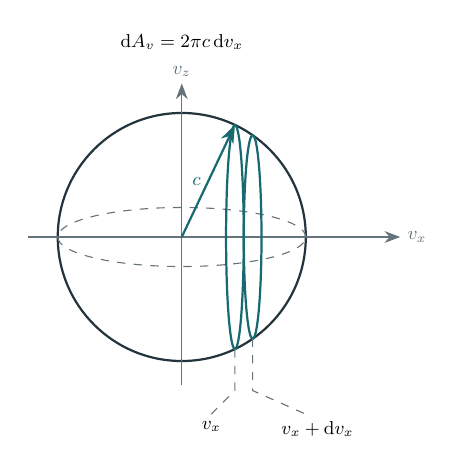
\begin{tikzpicture}[scale=.75,transform shape]

\draw[object] (0,0) circle (2.1);
\draw[guide] (0,0) ellipse (2.1 and .5);
\draw[axis] (-2.6,0)--(3.7,0) node[right] {$v_x$};
\draw[axis] (0,-2.5)--(0,2.6) node[above] {$v_z$};
\draw[traj] (.9,0) ellipse (.15 and 1.897);
\draw[traj] (1.2,0) ellipse (.15 and 1.723);
\draw[motion] (0,0)--(.9,1.897) node[midway,left] {$c$};
\draw[guide] (.9,-1.9)--(.9,-2.6)--(.5,-3.0);
\draw[guide] (1.2,-1.72)--(1.2,-2.6)--(2.1,-3);
\node[below] at (.5,-3) {$v_x$};
\node[below] at (2.3,-3) {$v_x+\mathrm dv_x$};
\node at (0,3.3) {$\mathrm dA_v=2\pi c\,\mathrm dv_x$};

\end{tikzpicture}
\figcaption{解图热试2.5D\quad 速度球面上等宽球带具有相同面积，分量分布为常量。}
\end{minipage}\end{center}
若$\mu=\cos\theta=v_x/c$，则球带面积为
\[
\mathrm dA_v=2\pi c^2\,\mathrm d\mu=2\pi c\,\mathrm dv_x.
\]
这个球带面积也可用圆周长解释：球带处的横截面半径为$\rho=\sqrt{c^2-v_x^2}$，圆周长为$2\pi\rho$；沿球面的带宽为$c\mathrm dv_x/\rho$，两者相乘后$\rho$约去，得到$2\pi c\mathrm dv_x$。因此等宽$\mathrm dv_x$的球带有相同面积，尽管它们的圆周长不同。除以球面总面积$4\pi c^2$即为概率：
\[
f(v_x)\,\mathrm dv_x=\frac{\mathrm dv_x}{2c}.
\]
因此
\[
\boxed{f(v_x)=
\begin{cases}
1/(2c),&-c\le v_x\le c,\\
0,&|v_x|>c.
\end{cases}}
\]
积分$\int_{-c}^c f(v_x)\,\mathrm dv_x=1$，且$\langle v_x^2\rangle=c^2/3$，与各向同性相符。

第（5）问，解图热试2.5E把孔外方向设为$v_x>0$。频段$\nu$中该速度分量区间内，每秒穿过单位孔面积的光子数是$n_\nu v_xf(v_x)\,\mathrm dv_x$，即该区间的数密度$n_\nu f(v_x)\mathrm dv_x$再乘法向速度$v_x$。因此
\[
J_\nu
=n_\nu h\nu\int_0^c v_x f(v_x)\,\mathrm dv_x
=u_\nu\int_0^c\frac{v_x}{2c}\,\mathrm dv_x
=\frac c4u_\nu.
\]
\begin{center}\begin{minipage}{.98\linewidth}\centering
\begin{tikzpicture}[scale=.85,transform shape]

\draw[object,line width=2pt] (0,-1.8)--(0,-.6);
\draw[object,line width=2pt] (0,.6)--(0,1.8);
\fill[accent!8] (-2.5,-.6) rectangle (0,.6);
\draw[guide] (-2.5,-.6)--(-2.5,.6);
\draw[motion] (-2, .3)--(1.3,.3) node[right] {$v_x>0$};
\draw[axis] (.2,-1)--(2,-1) node[right] {孔外};
\draw[axis,<->] (-2.5,-1)--(0,-1) node[midway,below] {$v_x\,\mathrm dt$};
\node[left] at (0,1.5) {腔内};
\node[right] at (.2,.9) {小孔};
\node at (0,-2.4) {$J=u\int_0^c v_xf(v_x)\,\mathrm dv_x=cu/4$};

\end{tikzpicture}
\figcaption{解图热试2.5E\quad 穿孔光子数按正的法向速度加权，积分只取出射半轴。}
\end{minipage}\end{center}
图E中速度区间内的光子在$\mathrm dt$内向外跨越厚度$v_x\mathrm dt$。单位孔面积前的这段体积内共有$n_\nu f(v_x)\mathrm dv_x\,v_x\mathrm dt$个光子，除以时间得到上述通量。只对$v_x>0$积分，既筛选出射方向，又按穿孔速度加权：
\[
\int_0^c v_x\frac{\mathrm dv_x}{2c}=\frac c4.
\]
这一系数在每个频段相同，故可以先求单频段再把能量密度相加。求和得
\[
\boxed{J=\frac c4u=\frac{ac}{4}T^4=\sigma T^4},
\qquad \sigma=\frac{ac}{4}.
\]
这里的$1/4$同时来自只取出射半空间和穿孔速度的投影加权。压强计算多一个法向动量因子，给$1/3$；两项角平均分别对应法向动量与穿孔能量。孔足够小且壁面继续维持热平衡，才能使用同一个内部$u(T)$计算连续辐射。\begin{center}\begin{minipage}{.98\linewidth}\centering
\begin{tikzpicture}[scale=.8,transform shape]
\draw[axis] (0,0)--(10.7,0) node[right] {$\mu=\cos\theta$};
\draw[axis] (0,0)--(0,3.2) node[above] {归一化角权重};
\node[above] at (5,3.5) {实线面积$p/u=1/3$，虚线面积$J/(cu)=1/4$};
\draw[traj] plot coordinates {(0.000000000,0.000000000) (0.083333333,0.000194444) (0.166666667,0.000777778) (0.250000000,0.001750000) (0.333333333,0.003111111) (0.416666667,0.004861111) (0.500000000,0.007000000) (0.583333333,0.009527778) (0.666666667,0.012444444) (0.750000000,0.015750000) (0.833333333,0.019444444) (0.916666667,0.023527778) (1.000000000,0.028000000) (1.083333333,0.032861111) (1.166666667,0.038111111) (1.250000000,0.043750000) (1.333333333,0.049777778) (1.416666667,0.056194444) (1.500000000,0.063000000) (1.583333333,0.070194444) (1.666666667,0.077777778) (1.750000000,0.085750000) (1.833333333,0.094111111) (1.916666667,0.102861111) (2.000000000,0.112000000) (2.083333333,0.121527778) (2.166666667,0.131444444) (2.250000000,0.141750000) (2.333333333,0.152444444) (2.416666667,0.163527778) (2.500000000,0.175000000) (2.583333333,0.186861111) (2.666666667,0.199111111) (2.750000000,0.211750000) (2.833333333,0.224777778) (2.916666667,0.238194444) (3.000000000,0.252000000) (3.083333333,0.266194444) (3.166666667,0.280777778) (3.250000000,0.295750000) (3.333333333,0.311111111) (3.416666667,0.326861111) (3.500000000,0.343000000) (3.583333333,0.359527778) (3.666666667,0.376444444) (3.750000000,0.393750000) (3.833333333,0.411444444) (3.916666667,0.429527778) (4.000000000,0.448000000) (4.083333333,0.466861111) (4.166666667,0.486111111) (4.250000000,0.505750000) (4.333333333,0.525777778) (4.416666667,0.546194444) (4.500000000,0.567000000) (4.583333333,0.588194444) (4.666666667,0.609777778) (4.750000000,0.631750000) (4.833333333,0.654111111) (4.916666667,0.676861111) (5.000000000,0.700000000) (5.083333333,0.723527778) (5.166666667,0.747444444) (5.250000000,0.771750000) (5.333333333,0.796444444) (5.416666667,0.821527778) (5.500000000,0.847000000) (5.583333333,0.872861111) (5.666666667,0.899111111) (5.750000000,0.925750000) (5.833333333,0.952777778) (5.916666667,0.980194444) (6.000000000,1.008000000) (6.083333333,1.036194444) (6.166666667,1.064777778) (6.250000000,1.093750000) (6.333333333,1.123111111) (6.416666667,1.152861111) (6.500000000,1.183000000) (6.583333333,1.213527778) (6.666666667,1.244444444) (6.750000000,1.275750000) (6.833333333,1.307444444) (6.916666667,1.339527778) (7.000000000,1.372000000) (7.083333333,1.404861111) (7.166666667,1.438111111) (7.250000000,1.471750000) (7.333333333,1.505777778) (7.416666667,1.540194444) (7.500000000,1.575000000) (7.583333333,1.610194444) (7.666666667,1.645777778) (7.750000000,1.681750000) (7.833333333,1.718111111) (7.916666667,1.754861111) (8.000000000,1.792000000) (8.083333333,1.829527778) (8.166666667,1.867444444) (8.250000000,1.905750000) (8.333333333,1.944444444) (8.416666667,1.983527778) (8.500000000,2.023000000) (8.583333333,2.062861111) (8.666666667,2.103111111) (8.750000000,2.143750000) (8.833333333,2.184777778) (8.916666667,2.226194444) (9.000000000,2.268000000) (9.083333333,2.310194444) (9.166666667,2.352777778) (9.250000000,2.395750000) (9.333333333,2.439111111) (9.416666667,2.482861111) (9.500000000,2.527000000) (9.583333333,2.571527778) (9.666666667,2.616444444) (9.750000000,2.661750000) (9.833333333,2.707444444) (9.916666667,2.753527778) (10.000000000,2.800000000)};
\draw[dashed,thick,color=warm] plot coordinates {(0.000000000,0.000000000) (0.083333333,0.011666667) (0.166666667,0.023333333) (0.250000000,0.035000000) (0.333333333,0.046666667) (0.416666667,0.058333333) (0.500000000,0.070000000) (0.583333333,0.081666667) (0.666666667,0.093333333) (0.750000000,0.105000000) (0.833333333,0.116666667) (0.916666667,0.128333333) (1.000000000,0.140000000) (1.083333333,0.151666667) (1.166666667,0.163333333) (1.250000000,0.175000000) (1.333333333,0.186666667) (1.416666667,0.198333333) (1.500000000,0.210000000) (1.583333333,0.221666667) (1.666666667,0.233333333) (1.750000000,0.245000000) (1.833333333,0.256666667) (1.916666667,0.268333333) (2.000000000,0.280000000) (2.083333333,0.291666667) (2.166666667,0.303333333) (2.250000000,0.315000000) (2.333333333,0.326666667) (2.416666667,0.338333333) (2.500000000,0.350000000) (2.583333333,0.361666667) (2.666666667,0.373333333) (2.750000000,0.385000000) (2.833333333,0.396666667) (2.916666667,0.408333333) (3.000000000,0.420000000) (3.083333333,0.431666667) (3.166666667,0.443333333) (3.250000000,0.455000000) (3.333333333,0.466666667) (3.416666667,0.478333333) (3.500000000,0.490000000) (3.583333333,0.501666667) (3.666666667,0.513333333) (3.750000000,0.525000000) (3.833333333,0.536666667) (3.916666667,0.548333333) (4.000000000,0.560000000) (4.083333333,0.571666667) (4.166666667,0.583333333) (4.250000000,0.595000000) (4.333333333,0.606666667) (4.416666667,0.618333333) (4.500000000,0.630000000) (4.583333333,0.641666667) (4.666666667,0.653333333) (4.750000000,0.665000000) (4.833333333,0.676666667) (4.916666667,0.688333333) (5.000000000,0.700000000) (5.083333333,0.711666667) (5.166666667,0.723333333) (5.250000000,0.735000000) (5.333333333,0.746666667) (5.416666667,0.758333333) (5.500000000,0.770000000) (5.583333333,0.781666667) (5.666666667,0.793333333) (5.750000000,0.805000000) (5.833333333,0.816666667) (5.916666667,0.828333333) (6.000000000,0.840000000) (6.083333333,0.851666667) (6.166666667,0.863333333) (6.250000000,0.875000000) (6.333333333,0.886666667) (6.416666667,0.898333333) (6.500000000,0.910000000) (6.583333333,0.921666667) (6.666666667,0.933333333) (6.750000000,0.945000000) (6.833333333,0.956666667) (6.916666667,0.968333333) (7.000000000,0.980000000) (7.083333333,0.991666667) (7.166666667,1.003333333) (7.250000000,1.015000000) (7.333333333,1.026666667) (7.416666667,1.038333333) (7.500000000,1.050000000) (7.583333333,1.061666667) (7.666666667,1.073333333) (7.750000000,1.085000000) (7.833333333,1.096666667) (7.916666667,1.108333333) (8.000000000,1.120000000) (8.083333333,1.131666667) (8.166666667,1.143333333) (8.250000000,1.155000000) (8.333333333,1.166666667) (8.416666667,1.178333333) (8.500000000,1.190000000) (8.583333333,1.201666667) (8.666666667,1.213333333) (8.750000000,1.225000000) (8.833333333,1.236666667) (8.916666667,1.248333333) (9.000000000,1.260000000) (9.083333333,1.271666667) (9.166666667,1.283333333) (9.250000000,1.295000000) (9.333333333,1.306666667) (9.416666667,1.318333333) (9.500000000,1.330000000) (9.583333333,1.341666667) (9.666666667,1.353333333) (9.750000000,1.365000000) (9.833333333,1.376666667) (9.916666667,1.388333333) (10.000000000,1.400000000)};
\node[below] at (0,-.12) {$0$};
\node[below] at (5,-.12) {$1/2$};
\node[below] at (10,-.12) {$1$};
\end{tikzpicture}
\figcaption{解图热试2.5F\quad 实线面积$p/u=1/3$，虚线面积$J/(cu)=1/4$}
\end{minipage}\end{center}
图F把法向方向余弦$\mu$从0到1的两项权重放在同一坐标中。压强的归一化积分是$\int_0^1\mu^2\mathrm d\mu=1/3$，孔流的归一化积分是$\int_0^1\mu\mathrm d\mu/2=1/4$，面积分别对应$p/u$和$J/(cu)$。因而$1/3$表示反射法向动量的平均，$1/4$表示出射能量的通量平均；两者共同使用内部各向同性的能量分布。



\end{document}
